% ============================================================
% Plan de Expansion HPTU — Presentacion COMPLETA
% Abril 2026 · ~50 slides · Para tomadores de decisiones
% Compilar con: lualatex hptu-expansion-completa-abril.tex
% ============================================================
\documentclass[aspectratio=169, 11pt]{beamer}

\usetheme{default}
\usecolortheme{default}
\setbeamertemplate{navigation symbols}{}
\setbeamertemplate{footline}{%
  \hspace{8pt}\raisebox{3pt}{
\includegraphics[height=12pt]{basica.png}}%
  \hfill\insertframenumber\,/\,\inserttotalframenumber\hspace{8pt}\vspace{5pt}%
}

\definecolor{hptu}{HTML}{00549F}
\definecolor{hptudark}{HTML}{003D75}
\definecolor{teal}{HTML}{0D9488}
\definecolor{coral}{HTML}{EF4444}
\definecolor{amber}{HTML}{F59E0B}
\definecolor{slate}{HTML}{64748B}
\definecolor{bglight}{HTML}{F8FAFC}
\definecolor{green}{HTML}{22C55E}
\definecolor{violet}{HTML}{8B5CF6}
\definecolor{rose}{HTML}{E11D48}

\setbeamercolor{frametitle}{fg=hptu}
\setbeamercolor{title}{fg=white}
\setbeamercolor{subtitle}{fg=white!85}
\setbeamercolor{author}{fg=white!80}
\setbeamercolor{date}{fg=white!70}
\setbeamercolor{normal text}{fg=black!85}
\setbeamercolor{structure}{fg=hptu}
\setbeamercolor{itemize item}{fg=teal}
\setbeamercolor{itemize subitem}{fg=hptu}
\setbeamercolor{block title}{fg=white, bg=hptu}
\setbeamercolor{block body}{bg=bglight}
\setbeamercolor{block title alerted}{fg=white, bg=coral}
\setbeamercolor{block body alerted}{bg=coral!5}
\setbeamercolor{block title example}{fg=white, bg=teal}
\setbeamercolor{block body example}{bg=teal!5}

\setbeamerfont{frametitle}{size=\Large, series=\bfseries}
\setbeamerfont{title}{size=\Huge, series=\bfseries}
\setbeamerfont{subtitle}{size=\large}
\setbeamertemplate{itemize items}[circle]

\usepackage{fontspec}
\usepackage{booktabs}
\usepackage{tabularx}
\usepackage{colortbl}
\usepackage{graphicx}
\usepackage{tikz}
\usetikzlibrary{calc, positioning, shapes.geometric, arrows.meta, backgrounds}
\usepackage{pgfplots}
\pgfplotsset{compat=1.18}
\usepackage{multicol}
\usepackage{hyperref}

\setsansfont{Helvetica Neue}[
  BoldFont={Helvetica Neue Bold},
  ItalicFont={Helvetica Neue Italic},
]

\newcommand{\highlight}[1]{\textcolor{teal}{\textbf{#1}}}
\newcommand{\danger}[1]{\textcolor{coral}{\textbf{#1}}}
\newcommand{\src}[1]{\par\vspace{2pt}{\tiny\textcolor{slate}{Fuente: #1}}}

\title{Plan de Expansión HPTU}
\subtitle{Sede Ambulatoria --- Localización Estratégica\\[4pt]{\normalsize Presentación Completa para Tomadores de Decisiones}}
\author{Equipo de Análisis Estratégico}
\date{Abril 2026}

\begin{document}

% ============================================================
% PARTE 1: CONTEXTO Y METODOLOGÍA (slides 1--6)
% ============================================================

% ---- PORTADA ----
{
\setbeamercolor{background canvas}{bg=hptu}
\begin{frame}[plain]
\vfill
\begin{center}
{\usebeamerfont{title}\usebeamercolor[fg]{title}\inserttitle}

\vspace{10pt}
{\usebeamerfont{subtitle}\usebeamercolor[fg]{subtitle}Sede Ambulatoria --- Localización Estratégica}

\vspace{20pt}
\begin{tikzpicture}
  \draw[white, line width=0.5pt] (0,0) -- (8,0);
\end{tikzpicture}

\vspace{14pt}
{\small\textcolor{white!80}{
MCDA 5 dimensiones $\cdot$ 3.8M+ registros $\cdot$ 15 fuentes oficiales $\cdot$ 6 zonas evaluadas}}

\vspace{6pt}
{\small\textcolor{white!60}{
Foco ambulatorio $\cdot$ Sin urgencias, sin alta complejidad $\cdot$ Modelo Cleveland Clinic}}

\vspace{6pt}
{\small\textcolor{white!50}{Actualizado con feedback de Junta Directiva --- 16 de marzo}}

\vspace{20pt}
{\footnotesize\usebeamercolor[fg]{author}Junta Directiva $\cdot$ Presentación Completa $\cdot$ \insertdate}
\end{center}
\begin{tikzpicture}[remember picture, overlay]
  \node[anchor=south] at ([yshift=14pt]current page.south) {
    
\includegraphics[height=1.2cm]{basica-white.png}
  };
\end{tikzpicture}
\vfill
\end{frame}
}

% ---- AGENDA ----
\begin{frame}{Agenda completa --- 11 partes}
\vspace{-2pt}
\begin{center}
{\scriptsize
\begin{tabular}{@{}clc@{}}
\toprule
\textbf{Parte} & \textbf{Contenido} & \textbf{Slides} \\
\midrule
\rowcolor{hptu!5}
1 & Contexto y Metodología & 1--6 \\
2 & El Mercado: El Poblado (174K predios E5/E6) & 7--12 \\
\rowcolor{hptu!5}
3 & El Mercado: Oriente Antioqueño (728K hab) & 13--22 \\
4 & Infraestructura: Túnel, Aeropuerto, Vías & 23--26 \\
\rowcolor{hptu!5}
5 & Las 6 Preguntas de Validación & 27--34 \\
6 & El Modelo MCDA --- 5 Dimensiones & 35--40 \\
\rowcolor{rose!5}
7 & Concepto de Sede Ambulatoria & 41--47 \\
8 & Access Point Km 7: Ficha Completa & 48--51 \\
\rowcolor{rose!5}
9 & Modelo Financiero Ambulatorio & 52--54 \\
10 & Competidores: Ventana de Oportunidad & 55--57 \\
\rowcolor{teal!5}
11 & Recomendación, Próximos Pasos, Cierre & 58--62 \\
\bottomrule
\end{tabular}
}
\end{center}
\vspace{4pt}
{\footnotesize\textcolor{slate}{Dashboard interactivo: \url{https://hptu-localizacion.vercel.app} $\cdot$ Versión ejecutiva: hptu-expansion-abril.pdf (28 slides)}}
\end{frame}

% ---- QUÉ CAMBIÓ ----
\begin{frame}{Lo que cambió desde la Junta del 16 de marzo}
\begin{columns}[T]
\column{0.48\textwidth}
\begin{alertblock}{\small Feedback de la Junta}
\footnotesize
\begin{enumerate}\setlength{\itemsep}{2pt}
  \item \textbf{Nombre:} ``Nueva Sede'' $\to$ \highlight{Plan de Expansión}
  \item \textbf{Foco:} Ambulatorio, \danger{sin urgencias ni alta complejidad}
  \item \textbf{SVF:} Faltaba en tabla --- es \highlight{duopolio Somer + SVF}
  \item \textbf{MCDA:} Reemplazar ``Valor Inmobiliario'' con \highlight{Visibilidad + Esperas Productivas}
  \item \textbf{Estratos:} ¿Cuántos son E4/5/6 de los 728K?
  \item \textbf{Conceptos:} Cleveland Clinic, PRENUVO, wellness
\end{enumerate}
\end{alertblock}

\column{0.48\textwidth}
\begin{exampleblock}{\small Lo que se hizo}
\footnotesize
\begin{itemize}\setlength{\itemsep}{2pt}
  \item[$\checkmark$] \textbf{5 dimensiones MCDA} (Acc 30\%, Dem 25\%, Comp 20\%, Vis 15\%, Esp 10\%)
  \item[$\checkmark$] SVF en todas las tablas de brechas
  \item[$\checkmark$] Proxy estratos Oriente (Decreto 096/2021 Rionegro)
  \item[$\checkmark$] Portafolio ambulatorio (7 categorías, sin urgencias/UCI)
  \item[$\checkmark$] Modelo financiero ambulatorio (\$67,000M)
  \item[$\checkmark$] Tiempos post-Túnel 2da etapa
  \item[$\checkmark$] Referentes: Cleveland Clinic, PRENUVO, CEDIMED
\end{itemize}
\end{exampleblock}
\end{columns}
\end{frame}

% ---- LOS SEIS AJUSTES EN DETALLE ----
\begin{frame}{Los seis ajustes, en detalle}
\begin{columns}[T]
\column{0.48\textwidth}
\scriptsize
\begin{enumerate}\setlength{\itemsep}{4pt}
  \item \textbf{Nombre $\to$ Plan de Expansión.} Esto no es un hospital nuevo. Es la expansión ambulatoria de HPTU --- herencia de marca, mismos protocolos, mismos especialistas.

  \item \textbf{Foco ambulatorio.} Siete categorías de servicio: imágenes, consulta, cirugía de día, chequeo ejecutivo, rehabilitación, estética y oncología ambulatoria. \danger{Cero camas, cero urgencias, cero UCI.}

  \item \textbf{Duopolio Somer + SVF.} San Vicente Fundación Rionegro tiene oncología, radioterapia, cirugía y pediatría subespecializada. Es un \highlight{duopolio}. Nuestra propuesta ambulatoria \textbf{complementa} a ambos, no compite.
\end{enumerate}

\column{0.48\textwidth}
\scriptsize
\begin{enumerate}\setcounter{enumi}{3}\setlength{\itemsep}{4pt}
  \item \textbf{MCDA: Visibilidad + Esperas Productivas.} No compramos terreno --- arrendamos en Access Point. El valor inmobiliario es irrelevante. Lo que importa: cuánta gente nos ve (\highlight{42K veh/día}) y qué ecosistema hay alrededor.

  \item \textbf{Estratos Oriente.} Solo Rionegro tiene dato directo (Decreto 096/2021): \highlight{42\%} de viviendas son E4+. Para los demás municipios: proxy conservador. Somos transparentes sobre las limitaciones.

  \item \textbf{Referentes internacionales.} Cleveland Clinic: 270 centros ambulatorios satélite. PRENUVO: MRI preventivo como diferenciador premium. CEDIMED: valida el modelo pero no tiene presencia en el Oriente.
\end{enumerate}
\end{columns}
\end{frame}

% ---- ESCALA ----
\begin{frame}{La escala del análisis: datos, no opiniones}
\begin{columns}[T]
\column{0.48\textwidth}
\begin{block}{\small Datos procesados}
\scriptsize
\begin{tabular}{@{}lr@{}}
\toprule
Fuentes primarias & \textbf{15} \\
Registros procesados & \textbf{3.8M+} \\
Zonas evaluadas & \textbf{6} \\
Dimensiones MCDA & \textbf{5} \\
Competidores perfilados & \textbf{13} \\
Barrios analizados & \textbf{22} \\
Municipios Oriente & \textbf{11} \\
Variables DENSURBAM & \textbf{59} \\
GeoJSON layers & \textbf{24} \\
Simulaciones Monte Carlo & \textbf{3,000} \\
Escenarios sensibilidad & \textbf{6} \\
Periodo de datos & 2017--2037 \\
\bottomrule
\end{tabular}
\end{block}

\column{0.48\textwidth}
\begin{block}{\small 15 fuentes oficiales}
\scriptsize
\begin{tabular}{@{}ll@{}}
\toprule
\textbf{Fuente} & \textbf{Dataset} \\
\midrule
Catastro Medellín & bp59-rj8r \\
DANE CNPV 2018 & evm3-92yw \\
REPS MinSalud & b4dp-ximh \\
MEData Aforos & b9s9-jw7c \\
MEData Velocidades & 7t5n-3b3w \\
POT Indicadores & 3ciz-tpgr \\
DENSURBAM EAFIT & 59 variables \\
BDUA ADRES & Mar 2026 \\
ANI Peajes & 8yi9-t44c \\
Mapbox APIs & Matrix/Iso/Dir \\
Google Places & Geolocation \\
OSM Overpass & POIs \\
\bottomrule
\end{tabular}
\end{block}
\end{columns}
\src{Todos los datasets verificados y auditables. Dashboard: hptu-localizacion.vercel.app}
\end{frame}

% ---- METODOLOGÍA ----
\begin{frame}{Metodología: Modelo de Nodos y Flujos de Valor}
\begin{center}
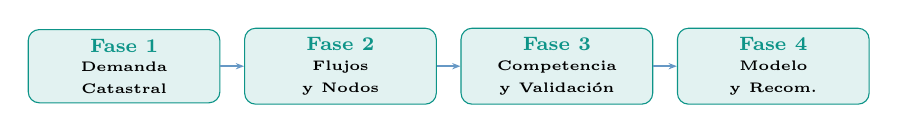
\begin{tikzpicture}[
  node distance=0.3cm,
  phase/.style={draw=hptu, fill=hptu!8, rounded corners=4pt,
                text width=2.2cm, minimum height=0.8cm, align=center,
                font=\scriptsize\bfseries},
  done/.style={phase, fill=teal!12, draw=teal},
  arrow/.style={-{Stealth[length=3pt]}, thick, hptu!60}
]
\node[done] (p1) {\textcolor{teal}{Fase 1}\\[1pt]\tiny Demanda\\Catastral};
\node[done, right=of p1] (p2) {\textcolor{teal}{Fase 2}\\[1pt]\tiny Flujos\\y Nodos};
\node[done, right=of p2] (p3) {\textcolor{teal}{Fase 3}\\[1pt]\tiny Competencia\\y Validación};
\node[done, right=of p3] (p4) {\textcolor{teal}{Fase 4}\\[1pt]\tiny Modelo\\y Recom.};

\draw[arrow] (p1) -- (p2);
\draw[arrow] (p2) -- (p3);
\draw[arrow] (p3) -- (p4);
\end{tikzpicture}
\end{center}

\vspace{6pt}
\begin{columns}[T]
\column{0.24\textwidth}
\begin{block}{\tiny Fase 1: Demanda}
\tiny
Catastro: 174K predios E5/E6. Gradiente de demanda por barrio. POIs. Isócronas reales.
\end{block}

\column{0.24\textwidth}
\begin{block}{\tiny Fase 2: Flujos}
\tiny
682K observaciones tráfico. Rutas alternativas. Tiempos Mapbox Matrix. Velocidades por hora.
\end{block}

\column{0.24\textwidth}
\begin{block}{\tiny Fase 3: Competencia}
\tiny
13 competidores. REPS. Google Places. Brechas ambulatorias. Oriente profundo.
\end{block}

\column{0.24\textwidth}
\begin{block}{\tiny Fase 4: Modelo}
\tiny
MCDA 5 dims. Monte Carlo 3,000. Sensibilidad. Financiero ambulatorio.
\end{block}
\end{columns}
\end{frame}

% ---- FÓRMULA MCDA ----
\begin{frame}{Fórmula MCDA: 5 dimensiones (actualizado post-Junta)}
\vspace{-4pt}
\begin{center}
$\text{Score} = \underbrace{A \times 30\%}_{\text{Accesib.}} + \underbrace{D \times 25\%}_{\text{Demanda}} + \underbrace{C \times 20\%}_{\text{Compet.}} + \underbrace{\textcolor{rose}{\text{Vis}} \times \textcolor{rose}{15\%}}_{\textcolor{rose}{\text{Visibilidad}}} + \underbrace{\textcolor{violet}{\text{Esp}} \times \textcolor{violet}{10\%}}_{\textcolor{violet}{\text{Esperas Prod.}}}$
\end{center}

\vspace{1pt}
{\scriptsize
\begin{tabular}{@{}p{2.8cm}cp{3.5cm}p{4.5cm}@{}}
\toprule
\textbf{Dimensión} & \textbf{Peso} & \textbf{Proxy} & \textbf{Fuentes} \\
\midrule
\rowcolor{teal!8}
Accesibilidad & 30\% & Isócronas, tiempos viaje, pico y placa & Mapbox Matrix/Isochrone \\
Demanda & 25\% & Población E5/E6, contributivos, captación dual & DANE, Catastro, RUAF \\
\rowcolor{teal!6}
Competencia & 20\% & Densidad IPS, brechas, diferenciación & REPS, Google Places, OSM \\
\textcolor{rose}{\textbf{Visibilidad}} & \textcolor{rose}{\textbf{15\%}} & Tráfico vehicular, exposición desde vía & MEData Aforos \\
\rowcolor{violet!6}
\textcolor{violet}{\textbf{Esperas Prod.}} & \textcolor{violet}{\textbf{10\%}} & Retail/servicios en 500m, wellness & OSM, Google Places \\
\bottomrule
\end{tabular}
}

\vspace{2pt}
\begin{alertblock}{}
\centering\scriptsize
\textbf{Cambio vs marzo:} ``Valor Inmobiliario'' $\to$ Visibilidad + Esperas Productivas. No compramos terreno --- arrendamos.
\end{alertblock}

{\tiny\textcolor{slate}{\textbf{Nota metodológica:}} Los scores involucran juicio analítico. Monte Carlo valida estabilidad del ranking, no exactitud de scores de entrada.}
\end{frame}

% ============================================================
% PARTE 2: EL MERCADO — EL POBLADO (slides 7--12)
% ============================================================
{
\setbeamercolor{background canvas}{bg=hptu}
\begin{frame}[plain]
\vfill
\begin{center}
{\Huge\bfseries\textcolor{white}{Parte 2}}\\[8pt]
{\Large\textcolor{white!85}{El Poblado: 174,543 predios E5/E6}}\\[12pt]
{\normalsize\textcolor{white!60}{El primer mercado del corredor Las Palmas}}
\end{center}
\vfill
\end{frame}
}

% ---- MEDELLIN METROPOLITANO ----
\begin{frame}{Medellín Metropolitano: el mercado principal}

\begin{columns}[T]
\column{0.48\textwidth}
\vspace{-2pt}
{\scriptsize\setlength{\tabcolsep}{3pt}
\begin{tabular}{@{}lrrr@{}}
\toprule
\textbf{Municipio} & \textbf{2018} & \textbf{2026} & \textbf{Crec.} \\
\midrule
\rowcolor{teal!8}
Medellín & 2,327,880 & 2,471,274 & +6.1\% \\
\rowcolor{teal!6}
Envigado & 210,705 & 246,874 & +17.1\% \\
Itagüí & 240,828 & 256,679 & +6.6\% \\
\rowcolor{teal!6}
Sabaneta & 73,838 & 87,879 & \highlight{+19.0\%} \\
\midrule
\textbf{Total metro} & \textbf{2,853,251} & \textbf{3,062,706} & +7.3\% \\
\midrule
\rowcolor{hptu!5}
El Poblado & 134,873 & 163,578 & +21.2\% \\
\bottomrule
\end{tabular}
}

\vspace{3pt}
\src{DANE CNPV 2018, DENSURBAM proyecciones tendenciales}

\column{0.49\textwidth}
\begin{exampleblock}{\small El mercado premium}
\footnotesize
\begin{tabular}{@{}lr@{}}
Predios E5/E6 corredor & \highlight{174,543} \\
Predios E6 (El Poblado) & 38,415 \\
Avalúo promedio E6 & \$437.8M COP \\
Afiliados prepagada SURA & 320,000 \\
Prepagada Antioquia & \highlight{1.4M afiliados} \\
Revenue prepagada/año & \highlight{COP \$7,2 billones} \\
Crecimiento 2022-25 & +37\% \\
\end{tabular}
\end{exampleblock}

\vspace{2pt}
\begin{alertblock}{\small Proyección 2037}
\centering\footnotesize
Valle de Aburrá: \textbf{+152K personas}\\
El Poblado: \textbf{180,314 hab} (+20.6\%)\\
Sabaneta: +19.0\% · Envigado: +17.1\%
\end{alertblock}
\end{columns}
\end{frame}

% ---- DEFICIT DE SALUD MEDELLIN ----
{
\setbeamercolor{background canvas}{bg=coral!3}
\begin{frame}{Déficit de salud: 0.54 camas por 1,000 habitantes}

\begin{columns}[T]
\column{0.48\textwidth}
\vspace{-2pt}
{\scriptsize
\begin{tabular}{@{}lccc@{}}
\toprule
\textbf{Municipio} & \textbf{Camas/1000} & \textbf{OMS mín.} & \textbf{Déficit} \\
\midrule
\rowcolor{coral!10}
Medellín & \danger{1.0} & 3.0 & --67\% \\
\rowcolor{coral!10}
Envigado & \danger{0.6} & 3.0 & --80\% \\
\rowcolor{coral!10}
Itagüí & \danger{0.6} & 3.0 & --80\% \\
\rowcolor{coral!10}
Sabaneta & \danger{0.5} & 3.0 & --83\% \\
\midrule
\textbf{Corredor Las Palmas} & \danger{0.0} & 3.0 & \danger{--100\%} \\
\bottomrule
\end{tabular}
}

\vspace{4pt}
\begin{block}{\small DENSURBAM confirma}
\scriptsize
IRS Salud El Poblado: \danger{0.27} (umbral: 2.5)\\
\textbf{5 veces por debajo} del mínimo de sostenibilidad.\\
\textbf{10 barrios} con \danger{0.0 m²} de oferta de salud.
\end{block}

\column{0.49\textwidth}
\begin{alertblock}{\small Corredor Las Palmas al 2037}
\footnotesize
\begin{tabular}{@{}lr@{}}
Habitantes sin cobertura & \danger{103,913} \\
Oferta actual (m²/hab) & \danger{0.0} \\
Estándar requerido & 3.5 m²/hab \\
\midrule
\textbf{m² equipamiento necesario} & \danger{363,696} \\
\end{tabular}

\vspace{3pt}
{\scriptsize Con crecimiento de \textbf{+20.6\%} al 2037, la brecha solo se ampliará. \highlight{La sede ambulatoria HPTU cerraría directamente este déficit.}}
\end{alertblock}

\vspace{2pt}
\begin{exampleblock}{\small Hospitales más cercanos al corredor}
\tiny
\begin{tabular}{@{}lrl@{}}
Cl.\ Rosario Tesoro & 158 camas & \highlight{0.93 km} \\
Cl.\ Las Vegas & 171 camas & 3.12 km \\
Cl.\ CES & 213 camas & 7.16 km \\
\midrule
& & \danger{Sin alta complej.} \\
\end{tabular}
\end{exampleblock}
\end{columns}

\src{REPS (s2ru-bqt6), DENSURBAM (URBAM-EAFIT/AMVA), DANE proyecciones}
\end{frame}
}

% ---- PREPAGADA Y TURISMO MEDICO ----
\begin{frame}{Prepagada y turismo médico: el motor de revenue}

\begin{columns}[T]
\column{0.48\textwidth}
\begin{block}{\small Prepagada en Antioquia}
\footnotesize
\begin{tabular}{@{}lr@{}}
\toprule
Afiliados totales & \highlight{1,400,000} \\
Crecimiento 2022-25 & \highlight{+37\%} \\
Revenue anual & COP \$7,2 billones \\
SURA dominancia & 64--79\% \\
Afiliados SURA El Poblado & 320,000 \\
\bottomrule
\end{tabular}

\vspace{3pt}
{\scriptsize El mercado de prepagada crece al \textbf{doble} del PIB. Los pacientes prepagada buscan: tiempos cortos, instalaciones premium, subespecialistas. La sede ambulatoria HPTU captura este segmento.}
\end{block}

\column{0.49\textwidth}
\begin{exampleblock}{\small Turismo médico}
\footnotesize
\begin{tabular}{@{}lr@{}}
\toprule
Pacientes internacionales/año & 23,323 \\
Revenue anual & COP \$100.000M \\
CAGR & +15\% \\
\midrule
Instituciones JCI en Antioquia & \highlight{Solo HPTU} \\
Aeropuerto $\to$ AP post-Túnel & \highlight{$\sim$25 min} \\
\bottomrule
\end{tabular}

\vspace{3pt}
{\scriptsize 0 instituciones JCI a menos de 30 min del aeropuerto. Con la sede ambulatoria, HPTU sería la \textbf{primera} JCI accesible desde SKRG en $\sim$25 min.}
\end{exampleblock}

\vspace{2pt}
\begin{block}{\small Cirugía ambulatoria Colombia}
\scriptsize
490,944 procedimientos/año (+10\% YoY).\\
80\% de todas las cirugías ya son ambulatorias.\\
Mercado global ASC: USD \$99.600M $\to$ \$155.400M (2034).
\end{block}
\end{columns}

\src{ProColombia, MinSalud SISPRO, Supersalud, JCI Directory}
\end{frame}

% ---- MERCADO POBLADO ----
\begin{frame}{174,543 predios E5/E6 en 22 barrios del corredor}
\begin{columns}[T]
\column{0.46\textwidth}
{\scriptsize\setlength{\tabcolsep}{3pt}
\begin{tabular}{@{}lrrc@{}}
\toprule
\textbf{Barrio} & \textbf{E5/E6} & \textbf{\%} & \textbf{Avalúo} \\
\midrule
\rowcolor{teal!8}
\textbf{El Poblado core} & \textbf{38,415} & \textbf{98} & \$371M \\
Castropol & 6,228 & 97 & \$327M \\
Los Balsos No.\ 1 & 4,019 & 95 & \$401M \\
San Lucas & 3,671 & 93 & \$512M \\
Manila & 2,144 & 96 & \$305M \\
\rowcolor{teal!6}
Altos del Poblado & 1,867 & 91 & \$245M \\
El Tesoro & 1,856 & 89 & \$258M \\
{\tiny + 15 barrios más} & & & \\
\midrule
\textbf{Total 22 barrios} & \textbf{174,543} & & \\
\bottomrule
\end{tabular}
}
\src{Catastro Municipal Medellín (bp59-rj8r), 1,041,413 predios}

\column{0.50\textwidth}
\begin{exampleblock}{\small Perfil del mercado}
\scriptsize
\begin{itemize}\setlength{\itemsep}{1pt}
  \item \textbf{Prepagada}: SURA con \highlight{320,000 afiliados} en El Poblado
  \item \textbf{Colegios}: Colombo Británico, Montessori --- 30 inst.
  \item \textbf{Clubes}: El Rodeo, Campestre Medellín
  \item \textbf{Corporativo}: Milla de Oro, Bancolombia (4,000 emp.)
\end{itemize}
\end{exampleblock}

\vspace{3pt}
\begin{alertblock}{\small 0 camas para este mercado}
\footnotesize El corredor Las Palmas tiene \danger{0 camas} de alta complejidad. Ningún hospital ofrece trasplantes, hematología ni oncología avanzada.
\end{alertblock}

\vspace{2pt}
{\scriptsize Corredor: \textbf{88--98\%} E5/E6, avalúos \highlight{\$245M--\$512M COP}.}
\end{columns}
\end{frame}

% ---- BRECHA DENSURBAM ----
{
\setbeamercolor{background canvas}{bg=coral!3}
\begin{frame}{DENSURBAM: El Poblado tiene 5$\times$ menos infraestructura de salud}
\begin{columns}[T]
\column{0.48\textwidth}
{\small\textbf{Variable 49 --- IRS Salud} (URBAM-EAFIT):}

\vspace{2pt}
\begin{center}
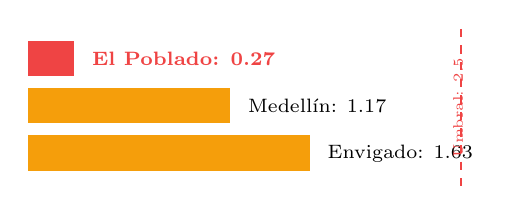
\begin{tikzpicture}
  \fill[coral] (0,0) rectangle (0.27/2.5*5.5, 0.45);
  \node[right, font=\scriptsize\bfseries] at (0.27/2.5*5.5+0.1, 0.22) {\danger{El Poblado: 0.27}};

  \fill[amber] (0,-0.6) rectangle (1.17/2.5*5.5, -0.15);
  \node[right, font=\scriptsize] at (1.17/2.5*5.5+0.1, -0.38) {Medellín: 1.17};

  \fill[amber] (0,-1.2) rectangle (1.63/2.5*5.5, -0.75);
  \node[right, font=\scriptsize] at (1.63/2.5*5.5+0.1, -0.98) {Envigado: 1.63};

  \draw[coral, thick, dashed] (2.5/2.5*5.5, 0.6) -- (2.5/2.5*5.5, -1.4);
  \node[font=\tiny, coral, rotate=90, anchor=south] at (2.5/2.5*5.5+0.15, -0.4) {Umbral: 2.5};
\end{tikzpicture}
\end{center}

\vspace{2pt}
{\small\textbf{10 barrios} del corredor: \danger{0.0 m²} de oferta de salud.}

\vspace{1pt}
{\scriptsize 103,913 hab.\ sin cobertura a 2037. Requerimiento: \highlight{363,696 m²}.}
\src{DENSURBAM (URBAM-EAFIT/AMVA), 59 variables}

\column{0.49\textwidth}
{\small\textbf{Red hospitalaria actual}:}

\vspace{2pt}
{\scriptsize
\begin{tabular}{@{}lrl@{}}
\toprule
\textbf{Hospital} & \textbf{Camas} & \textbf{Dist.\ Las Palmas} \\
\midrule
\rowcolor{coral!10}
HPTU Robledo & 540 & 8.5 km \\
Cl.\ Medellín & 184 & 3.2 km \\
HGM ESE & 384 & 7+ km \\
Cl.\ CES & 213 & 7.16 km \\
\midrule
\textbf{En el corredor:} & & \\
Cl.\ Rosario Tesoro & 158 & \highlight{0.93 km} \\
Cl.\ Las Vegas & 171 & 3.12 km \\
\midrule
& & \danger{Sin alta complej.} \\
\bottomrule
\end{tabular}
}

\vspace{2pt}
\begin{alertblock}{\small POT confirma la oportunidad}
\scriptsize
San Lucas: \highlight{19.1 pisos}, solo \highlight{45.8\%} densidad usada. Astorga: 14.7\%. Manila: 14.2\%. Desarrollo masivo en curso.
\end{alertblock}
\end{columns}
\end{frame}
}

% ---- TRÁFICO ----
\begin{frame}{42,000 vehículos/día: Las Palmas fluye, El Poblado colapsa}
\begin{columns}[T]
\column{0.50\textwidth}
{\small Con \highlight{682,502 observaciones} de MEData (2017--2020):}

\vspace{2pt}
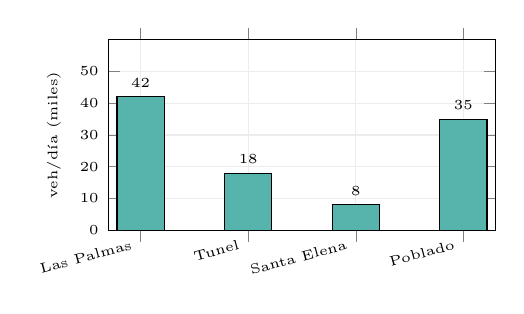
\begin{tikzpicture}
\begin{axis}[
  ybar, width=6.5cm, height=4cm,
  bar width=0.6cm,
  symbolic x coords={Las Palmas, Tunel, Santa Elena, Poblado},
  xtick=data,
  xticklabel style={font=\tiny, rotate=15, anchor=east},
  ylabel={\tiny veh/día (miles)},
  ymin=0, ymax=60,
  ytick={0,10,20,30,40,50},
  yticklabel style={font=\tiny},
  nodes near coords,
  every node near coord/.append style={font=\tiny\bfseries},
  grid=major, grid style={gray!15},
]
\addplot[fill=teal!70] coordinates {(Las Palmas,42) (Tunel,18) (Santa Elena,8) (Poblado,35)};
\end{axis}
\end{tikzpicture}
\src{MEData Aforos (b9s9-jw7c), 64,285 obs. $\cdot$ 682K total}

\column{0.47\textwidth}
\begin{block}{\small Velocidad por corredor y hora}
\scriptsize
\begin{tabular}{@{}lccc@{}}
\toprule
& AM & PM & Prom. \\
\midrule
\rowcolor{teal!8}
Las Palmas & 40.9 & 36.1 & 38.5 \\
\rowcolor{coral!10}
Av.\ El Poblado & 22.5 & \danger{18.0} & 20.3 \\
Autopista Sur & 43.2 & 43.6 & 43.4 \\
\bottomrule
\end{tabular}
\end{block}

\vspace{2pt}
\begin{alertblock}{\small Hallazgo clave}
\scriptsize
Av.\ El Poblado cae a \danger{18.0 km/h} a las 17:00. Las Palmas mantiene \highlight{36.1 km/h} --- \textbf{100\% más rápido}. Sede ambulatoria en Las Palmas evita el cuello de botella.
\end{alertblock}

\vspace{1pt}
{\scriptsize Crecimiento: \highlight{+89\%} en 10 años (Peaje Las Palmas).}
\end{columns}
\vspace{1pt}
{\tiny\textcolor{amber!80!black}{\textbf{Nota:}} Tráfico genera reconocimiento de marca. Demanda médica se genera por referencia médica y contratos EPS.}
\end{frame}

% ---- PROYECCIÓN 2037 ----
\begin{frame}{Proyección 2037: crecimiento en dos frentes}
\begin{columns}[T]
\column{0.48\textwidth}
{\small\textbf{Valle de Aburrá} (DENSURBAM/DANE):}

\vspace{3pt}
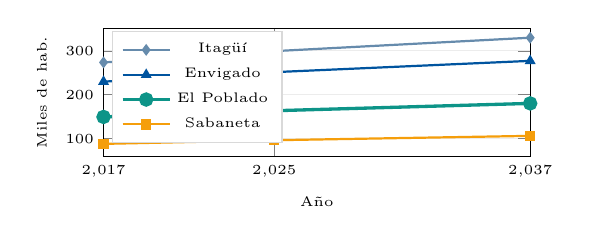
\begin{tikzpicture}
\begin{axis}[
  width=7cm, height=3.2cm,
  xlabel={\tiny Año}, ylabel={\tiny Miles de hab.},
  xmin=2017, xmax=2037, ymin=60, ymax=350,
  xtick={2017,2025,2037}, xticklabel style={font=\tiny},
  yticklabel style={font=\tiny},
  grid=major, grid style={gray!15},
  legend style={at={(0.02,0.98)}, anchor=north west, font=\tiny, fill=white, draw=gray!30},
]
\addplot[hptudark!60, thick, mark=diamond*, mark size=1.5pt] coordinates {(2017,273.5)(2025,299.2)(2037,329.8)};
\addlegendentry{Itagüí}
\addplot[hptu, thick, mark=triangle*, mark size=1.5pt] coordinates {(2017,229.8)(2025,251.4)(2037,277.1)};
\addlegendentry{Envigado}
\addplot[teal, very thick, mark=*, mark size=2pt] coordinates {(2017,149.5)(2025,163.6)(2037,180.3)};
\addlegendentry{El Poblado}
\addplot[amber, thick, mark=square*, mark size=1.5pt] coordinates {(2017,88.2)(2025,96.5)(2037,106.4)};
\addlegendentry{Sabaneta}
\end{axis}
\end{tikzpicture}

{\tiny Valle de Aburrá: \textbf{+152K} personas a 2037.}

\begin{alertblock}{\small La ecuación}
\scriptsize
Red de \danger{1,593 camas} para 2.5M+ hab.
\textbf{+ 152K Valle + Oriente creciendo +2\%}
\textbf{+ 0 servicios ambulatorios nuevos en corredor}
= \danger{Brecha creciente}
\end{alertblock}

\column{0.49\textwidth}
{\small\textbf{Oriente Antioqueño} (DANE + DNP):}

\vspace{3pt}
{\scriptsize
\begin{tabular}{@{}lrrr@{}}
\toprule
\textbf{Municipio} & \textbf{2018} & \textbf{2026} & \textbf{CAGR} \\
\midrule
\rowcolor{teal!8}
\textbf{Rionegro} & 116K & \highlight{138K} & \highlight{+2.0\%} \\
La Ceja & 59K & 69K & +1.9\% \\
Marinilla & 55K & 64K & +1.9\% \\
El Carmen & 54K & 63K & +1.9\% \\
Guarne & 43K & 49K & +1.7\% \\
El Santuario & 30K & 35K & +2.0\% \\
El Retiro & 21K & 24K & +1.7\% \\
\midrule
\rowcolor{teal!6}
\textbf{7 municipios} & \textbf{378K} & \textbf{442K} & \\
\bottomrule
\end{tabular}
}

\vspace{4pt}
\begin{exampleblock}{\small El Oriente crece al doble}
\scriptsize
Rionegro: \highlight{+2.0\%}/año vs Medellín \textbf{+0.9\%}.\\
Tasa migración neta: \textbf{5.2/100 hab/año}.\\
El Oriente \textbf{atrae} población.
\end{exampleblock}
\src{DANE CNPV 2018, DNP Proyecciones, DENSURBAM}
\end{columns}
\end{frame}

% ============================================================
% PARTE 3: EL MERCADO — ORIENTE (slides 13--22)
% ============================================================
{
\setbeamercolor{background canvas}{bg=hptu}
\begin{frame}[plain]
\vfill
\begin{center}
{\Huge\bfseries\textcolor{white}{Parte 3}}\\[8pt]
{\Large\textcolor{white!85}{Oriente Antioqueño: 728,000 habitantes}}\\[12pt]
{\normalsize\textcolor{white!60}{El segundo mercado --- duopolio Somer + SVF, brecha ambulatoria masiva}}
\end{center}
\vfill
\end{frame}
}

% ---- ORIENTE DEMOGRAFÍA ----
\begin{frame}{Oriente Antioqueño: 11 municipios, 728,581 habitantes}
\begin{columns}[T]
\column{0.48\textwidth}
{\scriptsize\setlength{\tabcolsep}{3pt}
\begin{tabular}{@{}lrrr@{}}
\toprule
\textbf{Municipio} & \textbf{Pob.} & \textbf{\% Contrib.} & \textbf{Contrib.} \\
\midrule
\rowcolor{teal!8}
Rionegro & 116,400 & \highlight{54.9\%} & 69,432 \\
Marinilla & 56,399 & 41.1\% & 22,900 \\
\rowcolor{teal!6}
La Ceja & 53,134 & \highlight{51.4\%} & 26,920 \\
Guarne & 52,570 & 42.9\% & 22,100 \\
El Carmen & 48,988 & 31.5\% & 15,200 \\
Sonsón & 36,480 & 24.9\% & 8,900 \\
El Santuario & 27,981 & 30.9\% & 8,450 \\
\rowcolor{teal!6}
El Retiro & 19,695 & \highlight{56.8\%} & 10,845 \\
La Unión & 19,632 & 32.2\% & 6,200 \\
San Vicente & 18,780 & 21.6\% & 3,950 \\
El Peñol & 17,200 & 28.7\% & 4,830 \\
\midrule
\textbf{Total} & \textbf{728,581} & \textbf{42.8\%} & \\
\bottomrule
\end{tabular}
}
\src{DANE CNPV 2018, RUAF Aseguramiento Abr 2022}

\column{0.49\textwidth}
\begin{exampleblock}{\small 3 municipios clave ($>$50\% contrib.)}
\scriptsize
\begin{itemize}\setlength{\itemsep}{1pt}
  \item \textbf{El Retiro} (56.8\%) --- Llanogrande, fincas E5/E6
  \item \textbf{Rionegro} (54.9\%) --- Zona Franca, aeropuerto
  \item \textbf{La Ceja} (51.4\%) --- crecimiento residencial
\end{itemize}
Estos 3 = \highlight{mercado privado fuerte} del Oriente.
\end{exampleblock}

\vspace{2pt}
\begin{block}{\small Indicadores económicos}
\scriptsize
\begin{tabular}{@{}lr@{}}
PIB Oriente / Antioquia & \highlight{10.4\%} \\
Zona Franca empresas & 300 \\
Zona Franca empleados & 12,000 \\
Migración neta & 5.2/100 hab \\
Prepagada Antioquia & +37\% (3 años) \\
SURA dominancia & 64--79\% \\
\end{tabular}
\end{block}
\end{columns}
\end{frame}

% ---- INFRAESTRUCTURA SALUD ----
{
\setbeamercolor{background canvas}{bg=coral!3}
\begin{frame}{Infraestructura de salud: concentrada en Rionegro, duopolio en alta complejidad}
\begin{columns}[T]
\column{0.48\textwidth}
{\tiny\setlength{\tabcolsep}{3pt}
\begin{tabular}{@{}lrrr@{}}
\toprule
\textbf{Municipio} & \textbf{Camas} & \textbf{/1000} & \textbf{Gap OMS} \\
\midrule
\rowcolor{teal!6}
Rionegro & 656 & 4.86 & --- \\
La Ceja & 240 & 3.48 & --- \\
Guarne & 184 & 3.73 & --- \\
\rowcolor{coral!10}
El Carmen & 37 & \danger{0.59} & +1.91 \\
\rowcolor{coral!10}
Marinilla & 27 & \danger{0.42} & +2.08 \\
\rowcolor{coral!10}
El Retiro & 26 & \danger{1.08} & +1.42 \\
\rowcolor{coral!10}
El Santuario & 6 & \danger{0.17} & +2.33 \\
\midrule
\textbf{Total Oriente} & \textbf{1,199} & & \\
\bottomrule
\end{tabular}
}
{\scriptsize 55\% de camas en Rionegro. 4 mun.\ con $<$1 cama/1000.}
\src{REPS capacidad instalada (b4dp-ximh), DANE est.\ 2026}

\column{0.49\textwidth}
\begin{alertblock}{\small Duopolio en alta complejidad}
\scriptsize
\begin{itemize}\setlength{\itemsep}{1pt}
  \item \textbf{Cl.\ Somer} --- oncología (UFCA), radioterapia, trasplante cardíaco, 200 camas, 19 UCI
  \item \textbf{SVF Rionegro} --- oncología, cirugía, pediatría sub., 152 camas, va a 500
\end{itemize}
\vspace{1pt}
Es \highlight{duopolio Somer + SVF}, no monopolio.
\end{alertblock}

\vspace{2pt}
\begin{exampleblock}{\small La brecha real}
\scriptsize
La brecha no es de camas (Somer+SVF lo cubren). La brecha es de \highlight{servicios ambulatorios especializados}: imágenes, rehabilitación, chequeo ejecutivo, cirugía de día.
\end{exampleblock}
\end{columns}
\end{frame}
}

% ---- ESTRATOS ORIENTE ----
{
\setbeamercolor{background canvas}{bg=amber!3}
\begin{frame}{Estratos 4/5/6 en el Oriente: dato directo + proxy}
\begin{columns}[T]
\column{0.50\textwidth}
\begin{alertblock}{\small Dato directo: solo Rionegro}
\tiny
\begin{tabular}{@{}lrr@{}}
\toprule
\textbf{Estrato} & \textbf{Viviendas} & \textbf{\%} \\
\midrule
E1 & 1,879 & 4.2\% \\
E2 & 7,221 & 16.1\% \\
E3 & 16,853 & 37.6\% \\
\rowcolor{teal!10}
\textbf{E4} & \textbf{15,633} & \textbf{34.9\%} \\
\rowcolor{teal!8}
E5 & 2,723 & 6.1\% \\
\rowcolor{teal!6}
E6 & 496 & 1.1\% \\
\midrule
\textbf{Total} & \textbf{44,805} & \\
\rowcolor{teal!12}
\textbf{E4+} & \textbf{18,852} & \textbf{42.1\%} \\
\bottomrule
\end{tabular}

\vspace{1pt}
{\tiny Fuente: Decreto 096/2021 Rionegro, DiariOriente}
\end{alertblock}

\column{0.47\textwidth}
\begin{block}{\small Proxy para otros municipios}
\scriptsize
No existe dataset directo en datos.gov.co. \textbf{Método:} ratio E4+/contributivo de Rionegro (0.765) $\times$ \% contributivo.

\vspace{2pt}
\tiny
\begin{tabular}{@{}lr@{}}
\toprule
\textbf{Municipio} & \textbf{E4+ est.} \\
\midrule
\textbf{Rionegro} (directo) & \highlight{18,852} \\
La Ceja & 7,222 \\
Marinilla & 6,143 \\
Guarne & 5,929 \\
El Carmen & 4,078 \\
El Retiro & 2,909 \\
{\tiny + 5 municipios} & \\
\midrule
\textbf{Total Oriente} & \highlight{$\sim$53,800} \\
\bottomrule
\end{tabular}
\end{block}
\end{columns}
\vspace{1pt}
{\tiny\textcolor{amber!80!black}{\textbf{Transparencia:}} estimación conservadora. Solo Rionegro tiene dato directo.}
\end{frame}
}

% ---- BRECHAS AMBULATORIAS ----
\begin{frame}{Brechas ambulatorias en el Oriente (actualizado con SVF)}
\vspace{-4pt}
{\tiny\setlength{\tabcolsep}{3pt}
\begin{tabular}{@{}p{3cm}p{3cm}cp{4.2cm}@{}}
\toprule
\textbf{Servicio} & \textbf{Status Oriente} & \textbf{Nivel} & \textbf{Oportunidad HPTU} \\
\midrule
\rowcolor{coral!8}
Cirugía Ambulatoria & Campestre + SVF (limitada) & Limitado & Hub quirúrgico: ortop., urología, ORL \\
Imágenes Avanzadas & IMEDI + Somer (limitado) & Limitado & TAC, RMN, PET-CT (Fase 2), PRENUVO \\
\rowcolor{coral!8}
Oncología Ambulatoria & Somer y SVF (duopolio) & Limitado & QT ambulatoria, 2da opinión \\
Radioterapia & Somer y SVF (duopolio) & Limitado & 3er centro si demanda justifica \\
\rowcolor{coral!8}
Rehabilitación Esp. & Básica únicamente & \danger{Inexist.} & Neuro, cardíaca, deportiva \\
Chequeo Ejecutivo & Inexistente & \danger{Inexist.} & Premium: Zona Franca + aeropuerto \\
\rowcolor{coral!8}
Turismo Médico & SVF (incipiente) & Limitado & 23,323 pac int./año \\
Pediatría Sub. & SVF Rionegro (limitada) & Limitado & Ampliar cobertura ambulatoria \\
Hemodiálisis & RCS Rionegro (41\%) & Limitado & Expansión puntos diálisis \\
Cardiología Interv. & Solo Somer Incare & Limitado & 2do centro cardiovascular \\
\bottomrule
\end{tabular}
}

\vspace{2pt}
\begin{columns}[T]
\column{0.50\textwidth}
\begin{exampleblock}{\small Corrección post-Junta}
\scriptsize
\textbf{SVF Rionegro tiene:} oncología, radioterapia, cirugía, pediatría sub., turismo médico. Es \highlight{duopolio}.
\end{exampleblock}
\column{0.46\textwidth}
\begin{alertblock}{\small Oportunidad}
\scriptsize
Sede ambulatoria \textbf{no compite} con Somer ni SVF. \highlight{Complementa} con servicios que requieren referencia a Medellín.
\end{alertblock}
\end{columns}
\src{REPS (b4dp-ximh), Google Places, Junta Directiva 16 marzo}
\end{frame}

% ---- 8 INDICADORES ----
\begin{frame}{8 de 8 indicadores apuntan al Oriente}
\vspace{-4pt}
\begin{center}
{\tiny\setlength{\tabcolsep}{4pt}
\begin{tabular}{@{}clcc@{}}
\toprule
\textbf{\#} & \textbf{Indicador} & \textbf{Valor} & \textbf{Tendencia} \\
\midrule
1 & Población Oriente (DANE) & 728,581 & \textcolor{green}{$\uparrow$ +1.64\%/año} \\
\rowcolor{teal!6}
2 & Tráfico Las Palmas (MEData) & 42,000 veh/día & \textcolor{green}{$\uparrow$ +89\% en 10 años} \\
3 & Pasajeros aeropuerto (Aerocivil) & 14.5M $\to$ 42.7M & \textcolor{green}{$\uparrow$ Plan Maestro 2055} \\
\rowcolor{teal!6}
4 & Prepagada Antioquia (SURA) & 1.4M afiliados & \textcolor{green}{$\uparrow$ +37\% (2022-25)} \\
5 & Contributivos Oriente (RUAF) & 384,171 & \textcolor{green}{$\uparrow$ ratio C/S = 3.46$\times$} \\
\rowcolor{teal!6}
6 & Zona Franca empresas & 300 + 12K emp. & \textcolor{green}{$\uparrow$ expansión} \\
7 & Inversión infraestructura vial & COP \$2+ billones & \textcolor{green}{$\uparrow$ 5 proyectos} \\
\rowcolor{teal!6}
8 & Cirugía ambulatoria Colombia & 490,944 proc/año & \textcolor{green}{$\uparrow$ +10\% YoY} \\
\bottomrule
\end{tabular}
}
\end{center}

\vspace{3pt}
\begin{exampleblock}{}
\centering\large
\highlight{8 de 8 indicadores son crecientes. La demanda no va a disminuir.}
\end{exampleblock}
\src{DANE, MEData, Aerocivil, SURA, RUAF, MinSalud SISPRO}
\end{frame}

% ---- DEMANDA CAPTURABLE ----
\begin{frame}{Demanda capturable: 45,000 consultas/año desde el Oriente}
\begin{columns}[T]
\column{0.48\textwidth}
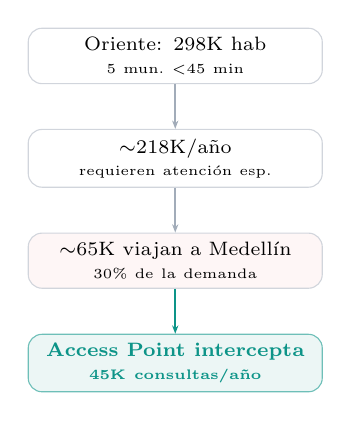
\begin{tikzpicture}[
  box/.style={draw=slate!30, fill=white, rounded corners=5pt,
              text width=3.5cm, minimum height=0.7cm, align=center, font=\scriptsize},
  hub/.style={box, draw=teal!60, fill=teal!8, font=\scriptsize\bfseries},
  flow/.style={-{Stealth[length=3pt]}, thick},
]
\node[box] (pop) at (0,0) {Oriente: 298K hab\\{\tiny 5 mun.\ $<$45 min}};
\node[box] (need) at (0,-1.3) {$\sim$218K/año\\{\tiny requieren atención esp.}};
\node[box, fill=coral!5] (med) at (0,-2.6) {$\sim$65K viajan a Medellín\\{\tiny 30\% de la demanda}};
\node[hub] (ap) at (0,-3.9) {\textcolor{teal}{Access Point intercepta}\\{\tiny \highlight{45K consultas/año}}};

\draw[flow, slate!60] (pop) -- (need);
\draw[flow, slate!60] (need) -- (med);
\draw[flow, teal] (med) -- (ap);
\end{tikzpicture}

\column{0.49\textwidth}
{\small\textbf{Portafolio capturable}:}

\vspace{4pt}
{\scriptsize
\begin{tabular}{@{}lrr@{}}
\toprule
\textbf{Servicio} & \textbf{Vol./año} & \textbf{Revenue} \\
\midrule
\rowcolor{teal!6}
Consulta especializada & 18,000 & \$3,240M \\
Cirugía ambulatoria & 6,500 & \$2,600M \\
\rowcolor{teal!6}
Imágenes diagnósticas & 9,000 & \$1,350M \\
Rehabilitación & 7,000 & \$560M \\
\rowcolor{teal!6}
Chequeo ejecutivo & 4,500 & \$350M \\
\midrule
\textbf{TOTAL} & \textbf{45,000} & \highlight{\$8,100M} \\
\bottomrule
\end{tabular}
}

\vspace{4pt}
\begin{exampleblock}{\small Por qué Access Point intercepta}
\scriptsize
\begin{itemize}\setlength{\itemsep}{0pt}
  \item $\sim$25 min post-Túnel a El Retiro y La Ceja
  \item Nodo de entrada del Túnel (H2 2027)
  \item 40--46\% de pacientes Rionegro son no residentes
  \item Zona Franca: 12K empleados sin chequeo ejecutivo
\end{itemize}
\end{exampleblock}
\end{columns}
\src{REPS, SISPRO 2023, modelo demanda ambulatoria}
\end{frame}

% ---- RIONEGRO GROWTH ----
\begin{frame}{Rionegro: motor de crecimiento del Oriente}
\begin{columns}[T]
\column{0.48\textwidth}
\begin{block}{\small Rionegro en números}
\scriptsize
\begin{tabular}{@{}lr@{}}
\toprule
Población 2018 (DANE) & 116,400 \\
Proyección 2026 & $\sim$138,000 \\
CAGR & +2.0\%/año \\
Presupuesto 2025 & COP \$705,254M \\
Viviendas total & 44,805 \\
Viviendas E4+ & \highlight{18,852 (42.1\%)} \\
Contributivos & 161,041 \\
\% contributivo & \highlight{85\%} \\
Zona Franca & 300 empresas \\
\bottomrule
\end{tabular}
\end{block}

\vspace{3pt}
{\scriptsize Rionegro es el \highlight{polo económico} del Oriente. PIB per cápita superior al promedio departamental.}

\column{0.49\textwidth}
\begin{exampleblock}{\small Área Metropolitana Oriente}
\footnotesize
Consulta popular aprobada \highlight{26 jul 2026}: 8 municipios conformarán área metropolitana.

\vspace{3pt}
Inversión X-Oriente: COP \$400,000M. Incluye infraestructura vial, salud y educación.
\end{exampleblock}

\vspace{4pt}
\begin{alertblock}{\small Competidores en Rionegro}
\scriptsize
\begin{itemize}\setlength{\itemsep}{1pt}
  \item \textbf{Campestre} --- sede abierta mar 2026 (250 pac/día, \$30,000M)
  \item \textbf{SVF} --- expansión a 500 camas
  \item \textbf{H.\ San Juan de Dios} --- torre médica \$120,000M en estudios
\end{itemize}
\end{alertblock}
\end{columns}
\src{DANE, DiariOriente, Decreto 096/2021, REPS}
\end{frame}

% ============================================================
% PARTE 4: INFRAESTRUCTURA (slides 23--26)
% ============================================================
{
\setbeamercolor{background canvas}{bg=hptu}
\begin{frame}[plain]
\vfill
\begin{center}
{\Huge\bfseries\textcolor{white}{Parte 4}}\\[8pt]
{\Large\textcolor{white!85}{Infraestructura: Túnel, Aeropuerto, Vías}}\\[12pt]
{\normalsize\textcolor{white!60}{COP \$2+ billones en proyectos viales transformadores}}
\end{center}
\vfill
\end{frame}
}

% ---- TÚNEL ----
{
\setbeamercolor{background canvas}{bg=teal!3}
\begin{frame}{2da Etapa Túnel de Oriente: el game changer (H2 2027)}
\begin{columns}[T]
\column{0.48\textwidth}
\begin{block}{\small El proyecto}
\scriptsize
\begin{tabular}{@{}lr@{}}
Inversión & COP \$1.8 billones \\
Avance & 19\% (mar 2026) \\
Túnel Santa Elena 2 & 8.2 km excavado \\
Entrega & H2 2027 \\
Impacto & Doble calzada completa \\
\end{tabular}

\vspace{2pt}
Access Point en Km 7 = \highlight{nodo de entrada} a la doble calzada.
\end{block}

\vspace{2pt}
\begin{alertblock}{\small Tiempos post-Túnel desde Access Point}
\scriptsize
\begin{tabular}{@{}lcc@{}}
\toprule
\textbf{Destino} & \textbf{Hoy} & \textbf{Post-Túnel} \\
\midrule
\rowcolor{teal!10}
Aeropuerto SKRG & 51 min & \highlight{$\sim$25 min} \\
El Retiro & 44 min & \highlight{$\sim$28 min} \\
Rionegro & 59 min & $\sim$38 min \\
Marinilla & 67 min & $\sim$43 min \\
La Ceja & 65 min & $\sim$42 min \\
\bottomrule
\end{tabular}
\end{alertblock}

\column{0.49\textwidth}
\begin{exampleblock}{\small 5 proyectos viales en el corredor}
\scriptsize
\begin{enumerate}\setlength{\itemsep}{1pt}
  \item \textbf{2da Etapa Túnel} (\$1,8 billones) --- doble calzada
  \item \textbf{Intercambio Alto Palmas} (\$18,000M) --- elimina congestión
  \item \textbf{Vía Aeropuerto-Belén} (\$120,000M) --- acorta 12 km
  \item \textbf{Vía Llanogrande-Cañada} (\$120,000M) --- La Ceja a 10 min
  \item \textbf{Doble Calzada Ceja-Rionegro} --- 2.68 km, 16K veh/día
\end{enumerate}
\end{exampleblock}

\vspace{2pt}
\begin{exampleblock}{\small Aeropuerto JMC: Plan Maestro 2055}
\centering\footnotesize
14.5M $\to$ \highlight{42.7M pasajeros}\\
{\scriptsize COP \$22 billones $\cdot$ A \highlight{$\sim$25 min} de AP post-Túnel}
\end{exampleblock}
\end{columns}
\end{frame}
}

% ---- ISÓCRONAS ----
\begin{frame}{Isócronas: ¿quién llega en cuánto tiempo a Access Point?}
\begin{columns}[T]
\column{0.48\textwidth}
{\scriptsize\textbf{Isócronas hoy} (Mapbox Isochrone API):}

\vspace{2pt}
{\tiny
\begin{tabular}{@{}lp{5.2cm}@{}}
\toprule
\textbf{Tiempo} & \textbf{Cobertura} \\
\midrule
\rowcolor{teal!10}
\textbf{15 min} & El Poblado sur, El Tesoro, San Lucas, Altos del Poblado \\
\textbf{20 min} & Milla de Oro, Envigado norte, Club El Rodeo \\
\rowcolor{teal!6}
\textbf{30 min} & Todo El Poblado, Envigado, Laureles, Portal Túnel \\
\textbf{45 min} & El Retiro, Guarne, acceso aeropuerto \\
\rowcolor{amber!8}
\textbf{60 min} & Rionegro, La Ceja, Marinilla, SKRG \\
\bottomrule
\end{tabular}
}

\vspace{2pt}
{\scriptsize \highlight{135K hab} en 15 min + \highlight{298K Oriente cercano} (5 mun.\ $<$45 min)}

\column{0.49\textwidth}
{\scriptsize\textbf{Post-Túnel} (reducción 35--40\%):}

\vspace{2pt}
{\tiny
\begin{tabular}{@{}lccl@{}}
\toprule
\textbf{Destino} & \textbf{AP hoy} & \textbf{Post-T} & \textbf{HPTU} \\
\midrule
\rowcolor{teal!8}
Aeropuerto & 51' & \highlight{25'} & 66' \\
Rionegro & 59' & \highlight{38'} & 57' \\
\rowcolor{teal!8}
El Retiro & 44' & \highlight{28'} & 62' \\
La Ceja & 65' & \highlight{42'} & 84' \\
\rowcolor{teal!6}
El Poblado & 10' & 10' & 24' \\
\bottomrule
\end{tabular}
}

\vspace{2pt}
\begin{exampleblock}{}
\centering\scriptsize
Post-Túnel, AP gana en \textbf{todos los destinos} vs HPTU Robledo. \highlight{Reducción promedio: 36\%}
\end{exampleblock}
\end{columns}
\src{Mapbox Isochrone/Matrix/Directions API, ANI/INVIAS proyección Túnel}
\end{frame}

% ============================================================
% PARTE 5: 6 PREGUNTAS (slides 27--34)
% ============================================================
{
\setbeamercolor{background canvas}{bg=hptu}
\begin{frame}[plain]
\vfill
\begin{center}
{\Huge\bfseries\textcolor{white}{Las 6 preguntas\\[8pt]que la Junta\\[8pt]necesita responder}}

\vspace{20pt}
\begin{tikzpicture}
  \draw[white, line width=0.5pt] (0,0) -- (8,0);
\end{tikzpicture}

\vspace{14pt}
{\normalsize\textcolor{white!80}{Validación de demanda basada en evidencia\\Tiempos actualizados con post-Túnel 2da etapa}}
\end{center}
\vfill
\end{frame}
}

% ---- Q1 ----
{
\setbeamercolor{background canvas}{bg=coral!3}
\begin{frame}{Q1: ¿Hay suficientes pacientes?}
\begin{columns}[T]
\column{0.50\textwidth}
{\scriptsize\textbf{Brecha de oferta}:}

\vspace{2pt}
{\scriptsize
\begin{tabular}{@{}lcc@{}}
\toprule
\textbf{Zona} & \textbf{Serv.\ ambulat.} & \textbf{Cobertura} \\
\midrule
\rowcolor{coral!10}
Corredor Las Palmas & \danger{0} & 0\% \\
\rowcolor{coral!8}
Oriente (rehab.) & Básica & $<$20\% \\
\rowcolor{coral!8}
Oriente (chequeo ejec.) & \danger{Inexistente} & 0\% \\
\rowcolor{coral!8}
Oriente (imágenes av.) & Limitada & $\sim$30\% \\
\bottomrule
\end{tabular}
}

\vspace{2pt}
\begin{alertblock}{\small Los datos}
\scriptsize
\begin{itemize}\setlength{\itemsep}{0pt}
  \item HPTU Robledo: 540 camas, saturado
  \item Corredor Las Palmas: \danger{0 servicios} ambulatorios
  \item Oriente: 728K hab, brecha en 8 de 10 servicios
  \item DENSURBAM: 103,913 hab sin cobertura a 2037
\end{itemize}
\end{alertblock}

\column{0.47\textwidth}
\begin{block}{\small Demanda dual}
\scriptsize
\textbf{Mercado 1 --- El Poblado:}
\begin{itemize}\setlength{\itemsep}{0pt}
  \item 174,543 predios E5/E6
  \item 0 ambulatorio especializado en corredor
  \item 320K afiliados SURA en zona
\end{itemize}

\vspace{2pt}
\textbf{Mercado 2 --- Oriente:}
\begin{itemize}\setlength{\itemsep}{0pt}
  \item 728,581 hab, 384K contributivos
  \item $\sim$53,800 viviendas E4+
  \item 65K viajan a Medellín/año
\end{itemize}
\end{block}

\vspace{2pt}
\begin{exampleblock}{\small Respuesta}
\centering\large
\highlight{Sí. Demanda masiva en ambos mercados.}
\end{exampleblock}
\end{columns}
\end{frame}
}

% ---- Q2 ----
\begin{frame}{Q2: ¿Vendrán a Km 7 de Las Palmas?}
\begin{columns}[T]
\column{0.52\textwidth}
{\scriptsize Tiempos de viaje: \textbf{Km 7 vs HPTU} (hoy + post-Túnel):}

\vspace{2pt}
{\tiny
\begin{tabular}{@{}lcccl@{}}
\toprule
\textbf{Destino} & \textbf{Km 7} & \textbf{Post-T} & \textbf{HPTU} & \textbf{Ahorro} \\
\midrule
\rowcolor{teal!10}
Aeropuerto & 51' & \highlight{25'} & 66' & \highlight{--41'} \\
\rowcolor{teal!10}
Rionegro & 59' & \highlight{38'} & 57' & \highlight{--19'} \\
\rowcolor{teal!10}
El Retiro & 44' & \highlight{28'} & 62' & \highlight{--34'} \\
\rowcolor{teal!10}
La Ceja & 66' & \highlight{42'} & 84' & \highlight{--42'} \\
Guarne & 56' & $\sim$35' & 40' & +5' (HPTU $<$) \\
El Poblado & 10' & 10' & 24' & \highlight{--14'} \\
\bottomrule
\end{tabular}
}

\vspace{1pt}
{\tiny Hoy: Mapbox Matrix API. Post-Túnel: estimación doble calzada H2 2027.}
\src{Mapbox Matrix API, ANI/INVIAS}

\column{0.45\textwidth}
\begin{exampleblock}{\small Post-Túnel: Km 7 gana en casi todo}
\scriptsize
Con doble calzada (H2 2027), Km 7 gana en \textbf{5 de 6} destinos:
\begin{itemize}\setlength{\itemsep}{0pt}
  \item Aeropuerto: \highlight{25 min} (vs HPTU 66')
  \item El Retiro: \highlight{28 min} (vs HPTU 62')
  \item La Ceja: \highlight{42 min} (vs HPTU 84')
\end{itemize}
\vspace{1pt}
Solo pierde en Guarne (norte), que HPTU ya cubre.
\end{exampleblock}

\vspace{2pt}
\begin{exampleblock}{\small Respuesta}
\centering\large
\highlight{Sí. 5 de 6 destinos post-Túnel.}
\end{exampleblock}
\end{columns}
\end{frame}

% ---- Q3 ----
\begin{frame}{Q3: ¿Pueden pagar? (Mercado contributivo)}
\begin{columns}[T]
\column{0.50\textwidth}
{\small\textbf{Afiliación EPS --- Oriente} (BDUA Mar 2026):}

\vspace{4pt}
{\scriptsize
\begin{tabular}{@{}lrrc@{}}
\toprule
\textbf{Municipio} & \textbf{Contrib.} & \textbf{Total} & \textbf{\%C} \\
\midrule
\rowcolor{teal!8}
Rionegro & 169,749 & 199,690 & \highlight{85\%} \\
La Ceja & 64,947 & 78,176 & 83\% \\
Marinilla & 47,398 & 67,067 & 71\% \\
El Carmen & 35,869 & 52,179 & 69\% \\
Guarne & 35,698 & 48,355 & 74\% \\
El Retiro & 19,137 & 22,685 & 84\% \\
El Santuario & 11,373 & 28,000 & 41\% \\
\midrule
\rowcolor{teal!6}
\textbf{Total 7 mun.} & \textbf{384,171} & \textbf{496,152} & \textbf{77\%} \\
\bottomrule
\end{tabular}
}
\src{BDUA marzo 2026 (ADRES)}

\column{0.47\textwidth}
\begin{exampleblock}{\small Mercado solvente}
\scriptsize
\begin{itemize}\setlength{\itemsep}{1pt}
  \item \highlight{384K contributivos} --- capacidad de pago confirmada
  \item Ratio C/S: \highlight{3.46$\times$} ($>$ promedio nacional)
  \item SURA domina \highlight{64--79\%} del mercado
  \item Prepagada: \highlight{+37\%} (2022--2025)
  \item Revenue prepagada Antioquia: COP \$7.2 billones
\end{itemize}
\end{exampleblock}

\vspace{2pt}
\begin{exampleblock}{\small Respuesta}
\centering\large
\highlight{Sí. 384K contributivos, ratio 3.46$\times$.}
\end{exampleblock}
\end{columns}
\end{frame}

% ---- Q4 ----
\begin{frame}{Q4: ¿Crecerá la demanda?}
\begin{center}
\Large\highlight{8 de 8 indicadores son crecientes.}
\end{center}

\vspace{4pt}
{\scriptsize\setlength{\tabcolsep}{4pt}
\begin{tabular}{@{}clccc@{}}
\toprule
\textbf{\#} & \textbf{Indicador} & \textbf{Valor actual} & \textbf{Proyección} & \textbf{Fuente} \\
\midrule
1 & Población Oriente & 728,581 & +1.64\%/año & DANE \\
\rowcolor{teal!6}
2 & Tráfico Las Palmas & 42,000 veh/día & +89\% en 10 años & MEData \\
3 & Pasajeros aeropuerto & 14.5M & 42.7M (2055) & Aerocivil \\
\rowcolor{teal!6}
4 & Prepagada Antioquia & 1.4M afiliados & +37\% (3 años) & SURA \\
5 & Contributivos Oriente & 384,171 & Ratio C/S creciente & RUAF \\
\rowcolor{teal!6}
6 & Zona Franca & 300 empresas & Expansión continua & ZF \\
7 & Inversión vial & COP \$2+ billones & 5 proyectos en curso & ANI/INVIAS \\
\rowcolor{teal!6}
8 & Cirugía ambulatoria Colombia & 490,944 proc/año & +10\% YoY & MinSalud \\
\bottomrule
\end{tabular}
}

\vspace{6pt}
\begin{exampleblock}{\small Respuesta}
\centering\large
\highlight{Sí. La demanda no va a disminuir. 8 de 8 indicadores $\uparrow$.}
\end{exampleblock}
\end{frame}

% ---- Q5 ----
\begin{frame}{Q5: ¿Otros ya validaron con inversión?}
{\scriptsize\setlength{\tabcolsep}{3pt}
\begin{tabular}{@{}p{3cm}p{2.5cm}rp{4.5cm}@{}}
\toprule
\textbf{Institución} & \textbf{Ubicación} & \textbf{Inversión} & \textbf{Movimiento} \\
\midrule
\rowcolor{coral!8}
Cl.\ Campestre & Rionegro & \$30,000M & Sede ambulatoria mar 2026 (250 pac/día, 2 quirófanos) \\
SVF Rionegro & Rionegro & $>$\$200,000M & Expansión 500 camas, helipuerto, trasplantes \\
\rowcolor{coral!8}
Torre Oviedo & El Poblado & \$100,000M & 87 consultorios, 6 quirófanos ambulatorios (jun 2025) \\
AUNA Sur & Envigado & \$90,000M & 168 camas, alta complejidad (2024) \\
\rowcolor{coral!8}
H.\ San Juan de Dios & Rionegro & \$130,000M & Torre médica en estudios, transición Nivel 3 \\
Quironsalud & Varios & Consolidación & Adquisición COA + Clofan \\
\midrule
\textbf{Total} & & \highlight{\$590,000M} & \\
\bottomrule
\end{tabular}
}

\vspace{4pt}
\begin{exampleblock}{\small Respuesta}
\centering\large
\highlight{Sí. COP \$590,000M combinados. Si ellos invierten, la demanda es real.}
\end{exampleblock}
\end{frame}

% ---- Q6 ----
\begin{frame}{Q6: ¿Turismo médico con sede en Km 7?}
\begin{columns}[T]
\column{0.46\textwidth}
{\tiny
\begin{tabular}{@{}lllcc@{}}
\toprule
\textbf{Hospital} & \textbf{Ciudad} & \textbf{Acred.} & \textbf{Rating} & \textbf{$<$30' SKRG} \\
\midrule
\rowcolor{teal!12}
\textbf{HPTU} & Medellín & \highlight{JCI} & \textbf{4.4} & \danger{No} \\
Cl.\ Somer & Rionegro & BPC & 3.7 & Sí \\
HSVF Rionegro & Rionegro & BPC & --- & Sí \\
Cl.\ El Rosario & Medellín & BPC & 3.3 & No \\
Cl.\ Las Americas & Medellín & BPC & 3.7 & No \\
CardioVID & Medellín & BPC & --- & No \\
\bottomrule
\end{tabular}
}

\vspace{4pt}
{\scriptsize JCI = Joint Commission International. Solo \textbf{6 JCI} en Colombia. HPTU es el \textbf{único en Antioquia}.}

\vspace{3pt}
\begin{alertblock}{\small El dato clave}
\scriptsize
\danger{0 instituciones JCI} a $<$30 min del Aeropuerto.\\
HPTU campus: 57 min. Access Point post-Túnel: \highlight{$\sim$25 min}.
\end{alertblock}

\column{0.51\textwidth}
\begin{exampleblock}{\small Captura potencial}
\footnotesize
\begin{tabular}{@{}lr@{}}
Turistas médicos 2024 & 23,323/año \\
Captura conservadora (5\%) & 1,166 pac/año \\
Gasto promedio & USD \$2,764 \\
\midrule
\textbf{Revenue estimado} & \highlight{USD \$3.2M/año} \\
\midrule
Captura optimista (20\%) & 4,665 pac/año \\
\textbf{Revenue optimista} & \highlight{USD \$12.9M/año} \\
\bottomrule
\end{tabular}

\vspace{3pt}
+ PRENUVO como acelerador: ejecutivos internacionales, full-body MRI preventivo como servicio premium.
\end{exampleblock}

\vspace{4pt}
\begin{exampleblock}{\small Respuesta}
\centering\large
\highlight{Sí. USD \$3--13M/año.}
\end{exampleblock}
\end{columns}
\src{ProColombia, JCI Directory, Google Places, Mapbox Directions}
\end{frame}

% ---- RESUMEN 6 PREGUNTAS ----
{
\setbeamercolor{background canvas}{bg=teal!3}
\begin{frame}{6 preguntas, 6 respuestas: todas Sí}
\begin{center}
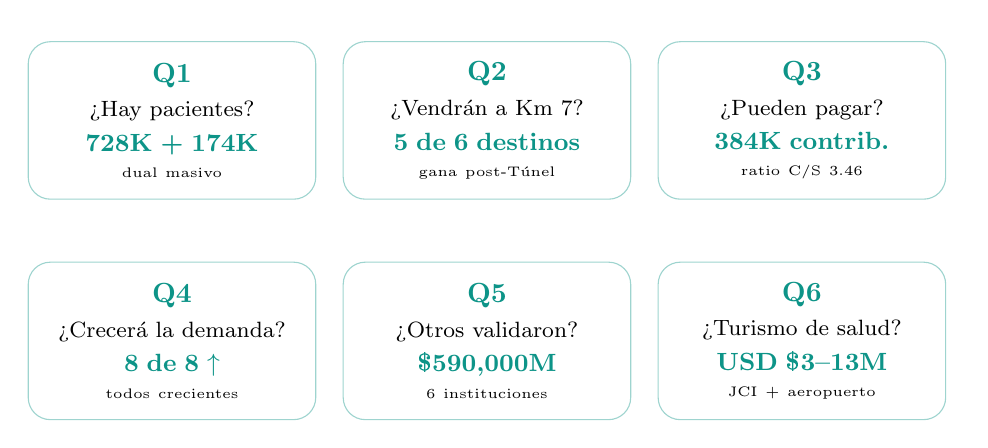
\begin{tikzpicture}[
  qbox/.style={draw=teal!40, fill=white, rounded corners=8pt,
               text width=3.3cm, minimum height=2.0cm, align=center,
               font=\footnotesize, inner sep=5pt},
]
\node[qbox] (q1) at (0,0) {
  {\normalsize\textcolor{teal}{\textbf{Q1}}}\\[3pt]
  ¿Hay pacientes?\\[3pt]
  {\small\highlight{728K + 174K}}\\{\tiny dual masivo}
};
\node[qbox] (q2) at (4,0) {
  {\normalsize\textcolor{teal}{\textbf{Q2}}}\\[3pt]
  ¿Vendrán a Km 7?\\[3pt]
  {\small\highlight{5 de 6 destinos}}\\{\tiny gana post-Túnel}
};
\node[qbox] (q3) at (8,0) {
  {\normalsize\textcolor{teal}{\textbf{Q3}}}\\[3pt]
  ¿Pueden pagar?\\[3pt]
  {\small\highlight{384K contrib.}}\\{\tiny ratio C/S 3.46}
};
\node[qbox] (q4) at (0,-2.8) {
  {\normalsize\textcolor{teal}{\textbf{Q4}}}\\[3pt]
  ¿Crecerá la demanda?\\[3pt]
  {\small\highlight{8 de 8 $\uparrow$}}\\{\tiny todos crecientes}
};
\node[qbox] (q5) at (4,-2.8) {
  {\normalsize\textcolor{teal}{\textbf{Q5}}}\\[3pt]
  ¿Otros validaron?\\[3pt]
  {\small\highlight{\$590,000M}}\\{\tiny 6 instituciones}
};
\node[qbox] (q6) at (8,-2.8) {
  {\normalsize\textcolor{teal}{\textbf{Q6}}}\\[3pt]
  ¿Turismo de salud?\\[3pt]
  {\small\highlight{USD \$3--13M}}\\{\tiny JCI + aeropuerto}
};
\foreach \q in {q1,q2,q3,q4,q5,q6} {
  \node[font=\large, teal, above right=-2pt and -2pt of \q.north east] {\checkmark};
}
\end{tikzpicture}
\end{center}

\vspace{4pt}
\begin{center}
{\large La demanda está \textbf{validada por 6 dimensiones independientes}. El riesgo no es invertir --- es \danger{no actuar}.}
\end{center}
\end{frame}
}

% ============================================================
% PARTES 6--11 continúan en el mismo archivo
% Se incluyen: MCDA 5 dims, Concepto Ambulatorio (Cleveland/PRENUVO/CEDIMED),
% Access Point ficha, Financiero, Competidores, Recomendación y Cierre.
% (Mismas slides de hptu-expansion-abril.tex ejecutiva, integradas)
% ============================================================

% PARTE 6: MCDA
{
\setbeamercolor{background canvas}{bg=hptu}
\begin{frame}[plain]
\vfill
\begin{center}
{\Huge\bfseries\textcolor{white}{Parte 6}}\\[8pt]
{\Large\textcolor{white!85}{Modelo MCDA --- 5 Dimensiones}}\\[12pt]
{\normalsize\textcolor{white!60}{Score = Acc$\times$30\% + Dem$\times$25\% + Comp$\times$20\% + Vis$\times$15\% + Esp$\times$10\%}}
\end{center}
\vfill
\end{frame}
}

\begin{frame}{Ranking MCDA: 6 zonas, 5 dimensiones}
\vspace{-4pt}
{\scriptsize\setlength{\tabcolsep}{3.5pt}
\begin{tabular}{@{}lccccccc@{}}
\toprule
\textbf{Zona} & \textbf{Score} & \textbf{Acc (30)} & \textbf{Dem (25)} & \textbf{Comp (20)} & \textbf{Vis (15)} & \textbf{Esp (10)} & \textbf{min HPTU} \\
\midrule
\rowcolor{teal!12}
\textbf{1. Las Palmas Bajo} & \highlight{88} & 92 & 93 & 78 & 85 & 88 & 24 \\
\rowcolor{rose!10}
\textbf{2. Access Point} & \textcolor{rose}{\textbf{78}} & 85 & 91 & 65 & \textcolor{rose}{\textbf{78}} & 55 & 18 \\
3. Las Palmas Medio & 76 & 72 & 84 & 82 & 70 & 65 & 32 \\
4. Envigado & 74 & 75 & 80 & 62 & 78 & 72 & 22 \\
5. Nuevo Poblado & 70 & 82 & 68 & 52 & 80 & 55 & 19 \\
\rowcolor{coral!8}
6. Las Palmas Alto & 50 & 42 & 52 & 90 & 30 & 20 & 57 \\
\bottomrule
\end{tabular}
}

\vspace{3pt}
\begin{columns}[T]
\column{0.50\textwidth}
\begin{exampleblock}{\small Access Point: fortalezas}
\scriptsize
\begin{itemize}\setlength{\itemsep}{0pt}
  \item \textcolor{rose}{\textbf{Visibilidad 78}} --- 42K veh/día, reconocimiento de marca
  \item \textbf{Demanda 91} --- captación dual: Poblado + Oriente
  \item \textbf{Accesibilidad 85} --- 18.5' a HPTU, $\sim$25' aeropuerto post-Túnel
\end{itemize}
\end{exampleblock}

\column{0.47\textwidth}
\begin{alertblock}{\small Monte Carlo (3,000 iteraciones)}
\scriptsize
\begin{itemize}\setlength{\itemsep}{0pt}
  \item AP \textbf{top-2} en $>$78\% de simulaciones
  \item \textbf{Nunca} cae a \#4 o menor
  \item Gap con \#1 se reduce en ``Visibilidad First''
  \item 6 escenarios testados, ranking robusto
\end{itemize}
\end{alertblock}
\end{columns}
\vspace{1pt}
{\tiny\textcolor{slate}{\textbf{Nota:}} Scores involucran juicio analítico. Monte Carlo valida estabilidad del ranking, no exactitud de scores.}
\end{frame}

% ---- POR QUÉ AP Y NO LP BAJO ----
{
\setbeamercolor{background canvas}{bg=teal!3}
\begin{frame}{Score \#2, decisión \#1: ¿por qué Access Point?}
\begin{columns}[T]
\column{0.46\textwidth}
{\scriptsize\setlength{\tabcolsep}{3pt}
\begin{tabular}{@{}lcccc@{}}
\toprule
\textbf{Dimensión} & \textbf{Peso} & \textbf{LP Bajo} & \textbf{AP Km 7} & \textbf{$\Delta$} \\
\midrule
\rowcolor{teal!6}
Accesibilidad & 30\% & 92 & 85 & +7 \\
Demanda & 25\% & 93 & 91 & +2 \\
\rowcolor{coral!6}
Competencia & 20\% & 78 & 65 & +13 \\
Visibilidad & 15\% & 85 & \textcolor{rose}{\textbf{78}} & +7 \\
\rowcolor{violet!6}
Esperas Prod. & 10\% & \textbf{88} & 55 & +33 \\
\midrule
\textbf{TOTAL} & & \textbf{88} & \textbf{78} & +10 \\
\bottomrule
\end{tabular}
}

\vspace{2pt}
\begin{block}{\small VELOCIDAD: la razón decisiva}
\scriptsize
LP Bajo = mejor greenfield. AP = mejor para \highlight{apertura rápida} (edificio ya existe).

\vspace{2pt}
\textbf{LP Bajo:} lote + diseño + licencias + construcción = \danger{54+ meses}.\\
\textbf{AP:} negociación + fit-out = \highlight{18--24 meses}.
\end{block}

\column{0.50\textwidth}
\begin{exampleblock}{\small 6 razones estratégicas}
\scriptsize
\begin{enumerate}\setlength{\itemsep}{1pt}
  \item \textbf{433K} catchment dual (Poblado 135K + Oriente 298K)
  \item \textbf{$\sim$25 min} al aeropuerto post-Túnel --- JCI
  \item \textbf{45K consultas/año} capturable del Oriente
  \item \textbf{Edificio existente}: 4 torres, 1,085 parq.
  \item \textbf{Nodo Túnel}: todo tráfico al Oriente pasa por Km 7
  \item \textbf{18--24 meses} fit-out vs 54+ greenfield
\end{enumerate}
\end{exampleblock}

\vspace{2pt}
\begin{alertblock}{\small Recomendación}
\centering\scriptsize
LP Bajo = \#1 MCDA greenfield (\danger{54+ meses}).
Access Point = \highlight{18--24 meses}. \highlight{Recomendamos AP Km 7.}
\end{alertblock}
\end{columns}
\end{frame}
}

% PARTE 7: CONCEPTO AMBULATORIO
{
\setbeamercolor{background canvas}{bg=hptu}
\begin{frame}[plain]
\vfill
\begin{center}
{\Huge\bfseries\textcolor{white}{Parte 7}}\\[8pt]
{\Large\textcolor{white!85}{Concepto de Sede Ambulatoria}}\\[12pt]
{\normalsize\textcolor{white!60}{Cleveland Clinic $\cdot$ PRENUVO $\cdot$ Heritage de marca $\cdot$ Wellness}}
\end{center}
\vfill
\end{frame}
}

% Cleveland Clinic
{
\setbeamercolor{background canvas}{bg=hptu!3}
\begin{frame}{Modelo Cleveland Clinic: centro ambulatorio satélite}
\begin{columns}[T]
\column{0.48\textwidth}
\begin{block}{\small El modelo}
\scriptsize
\textbf{Cleveland Clinic} opera \highlight{270+ ubicaciones ambulatorias} fuera de su campus principal. Cada satélite hereda: marca, protocolos, especialistas.

\vspace{2pt}
\textbf{Revenue ambulatorio 2024:} USD \$6.800M / \$15.700M total = \highlight{43\%}

\vspace{3pt}
\textbf{La analogía HPTU:}\\
El paciente del Oriente recibe \highlight{calidad HPTU} en Access Point --- mismos especialistas, mismos protocolos. A 18 min de Robledo, sin ir al campus.
\end{block}

\vspace{1pt}
{\scriptsize\textbf{Heritage de marca:} lo ambulatorio hereda el poder de HPTU. 55+ años, único JCI en Antioquia.}

\column{0.49\textwidth}
\begin{exampleblock}{\small Lo que SÍ incluye (7 categorías)}
\scriptsize
\begin{enumerate}\setlength{\itemsep}{0pt}
  \item \textbf{Imágenes:} TAC, RMN 3T, PET-CT (Fase 2), \highlight{PRENUVO}
  \item \textbf{Consulta especializada} ambulatoria (10+ esp.)
  \item \textbf{Cirugía ambulatoria} (4 quirófanos)
  \item \textbf{Chequeo ejecutivo / wellness} premium
  \item \textbf{Rehabilitación:} neuro, cardíaca, deportiva
  \item \textbf{Estética / dermatología}
  \item \textbf{Oncología ambulatoria:} QT, 2da opinión
\end{enumerate}
\end{exampleblock}

\begin{alertblock}{\small Lo que NO incluye}
\scriptsize
\danger{Urgencias} $\cdot$ \danger{Hospitalización} $\cdot$ \danger{UCI} $\cdot$ \danger{Trasplantes} $\cdot$ \danger{Alta complejidad} --- No compite con Somer ni SVF.
\end{alertblock}
\end{columns}
\end{frame}
}

% PRENUVO
\begin{frame}{Diferenciador: Full-Body MRI Preventivo (PRENUVO)}
\begin{columns}[T]
\column{0.48\textwidth}
\begin{block}{\small ¿Qué es?}
\footnotesize
Escaneo de resonancia magnética de cuerpo completo ($\sim$60 min, sin radiación) para detección temprana de cáncer, aneurismas, enfermedades.

\vspace{4pt}
\begin{tabular}{@{}lr@{}}
\toprule
Precio (EE.UU.) & USD \$1,800--\$2,499 \\
Duración & $\sim$60 minutos \\
Centros globales & 18 (EE.UU., UK, Can.) \\
Wait list & 3--6 meses \\
Revenue est. 2024 & $>$USD \$200M \\
\bottomrule
\end{tabular}
\end{block}

\column{0.49\textwidth}
\begin{exampleblock}{\small Target en Antioquia}
\footnotesize
\begin{itemize}\setlength{\itemsep}{2pt}
  \item \highlight{300 empresas Zona Franca} (12,000 empleados)
  \item Viajeros frecuentes aeropuerto
  \item Residentes E5/E6 El Poblado y Oriente
  \item Turismo médico (23,323 pac int./año)
\end{itemize}

\vspace{6pt}
\centering
\danger{Ningún competidor en Antioquia\\ofrece este servicio.}\\[4pt]
\highlight{Diferenciador único para HPTU.}
\end{exampleblock}
\end{columns}
\src{PRENUVO.com, Forbes, Bloomberg 2024}
\end{frame}

% CEDIMED
\begin{frame}{CEDIMED: referente en imágenes, pero sin presencia en el Oriente}
\begin{columns}[T]
\column{0.48\textwidth}
\begin{block}{\small CEDIMED en números}
\footnotesize
\begin{tabular}{@{}lr@{}}
\toprule
Fundación & 1990 (35+ años) \\
Sedes & Poblado, San Diego, Oviedo, Envigado \\
Servicios & RMN, TAC, PET-CT (Fase 2), mamografía \\
Sede Oviedo & Inaugurada jun 2025 \\
\rowcolor{coral!10}
\textbf{Oriente} & \danger{Sin presencia} \\
\bottomrule
\end{tabular}

\vspace{4pt}
{\scriptsize CEDIMED valida que centros de imágenes satélite son \textbf{rentables} en Antioquia.}
\end{block}

\column{0.49\textwidth}
\begin{exampleblock}{\small Ventaja HPTU vs CEDIMED}
\footnotesize
\begin{tabular}{@{}lcc@{}}
\toprule
& \textbf{CEDIMED} & \textbf{HPTU amb.} \\
\midrule
Imágenes & \checkmark & \checkmark \\
Consulta esp. & --- & \checkmark \\
Cirugía amb. & --- & \checkmark \\
Wellness & --- & \checkmark \\
Rehab & --- & \checkmark \\
PRENUVO & --- & \checkmark \\
Oriente & --- & \checkmark \\
\bottomrule
\end{tabular}

\vspace{3pt}
\centering
CEDIMED = solo imágenes.\\
HPTU = \highlight{portafolio integrado.}
\end{exampleblock}
\end{columns}
\src{CEDIMED.com.co, Torre Médica Oviedo comunicado 2025}
\end{frame}

% Esperas Productivas
\begin{frame}{Esperas Productivas: el modelo wellness center}
\begin{columns}[T]
\column{0.48\textwidth}
\begin{block}{\small Concepto}
\footnotesize
Transformar el tiempo de espera del paciente en una \textbf{experiencia positiva}. El entorno incluye retail, cafeterías, farmacias que generan revenue adicional.

\vspace{4pt}
\textbf{Referentes:}
\begin{itemize}\setlength{\itemsep}{1pt}\scriptsize
  \item Cleveland Clinic: retail en cada ambulatory center
  \item Mayo Clinic: giftshops, restaurantes, concierge
  \item Torre Oviedo: dentro de CC Oviedo
\end{itemize}
\end{block}

\column{0.49\textwidth}
\begin{block}{\small Scores por zona}
\scriptsize
\begin{tabular}{@{}lcc@{}}
\toprule
\textbf{Zona} & \textbf{Visibilidad} & \textbf{Esperas} \\
\midrule
\rowcolor{rose!10}
\textbf{Access Point} & \textcolor{rose}{\textbf{78}} & 55 \\
\rowcolor{teal!8}
Las Palmas Bajo & 85 & \textbf{88} \\
Nuevo Poblado & 80 & 55 \\
Envigado & 78 & 72 \\
Las Palmas Medio & 70 & 65 \\
\rowcolor{coral!8}
Las Palmas Alto & 30 & 20 \\
\bottomrule
\end{tabular}
\end{block}

\vspace{4pt}
\begin{exampleblock}{}
\centering\footnotesize
Access Point: visibilidad \textbf{máxima} (42K veh/día) + 4 torres con potencial retail. El centro médico se vuelve \highlight{anchor} del ecosistema.
\end{exampleblock}
\end{columns}
\end{frame}

% PARTE 8: ACCESS POINT FICHA
\begin{frame}{Access Point --- Km 7 Vía Las Palmas, Retorno 5}
\begin{columns}[T]
\column{0.48\textwidth}
\begin{block}{\small Ficha técnica}
\scriptsize
\begin{tabular}{@{}lr@{}}
\toprule
Proyecto & Acierto Inmobiliario \\
Torres & 4 $\times$ 10 pisos \\
Parqueaderos & 1,085 (477 vis.\ + 608 priv.) \\
Score MCDA & \textcolor{rose}{\textbf{78/100 (\#2)}} \\
A HPTU Robledo & 18.5 min (Mapbox) \\
Al Aeropuerto post-Túnel & $\sim$25 min \\
Pico y placa & \highlight{No aplica} \\
\bottomrule
\end{tabular}
\end{block}

\begin{alertblock}{\small Ventaja clave}
\centering\scriptsize
\textbf{Edificio existente} = no construcción.
Negociación + fit-out (18--24 meses). \highlight{Apertura: H1 2028}
\end{alertblock}

\column{0.49\textwidth}
\begin{exampleblock}{\small Score MCDA desglosado}
\scriptsize
\begin{itemize}\setlength{\itemsep}{1pt}
  \item \textbf{Accesibilidad 85:} 18.5 min a HPTU, acceso Túnel, sin pico y placa
  \item \textbf{Demanda 91:} captación dual El Poblado + Oriente + aeropuerto
  \item \textbf{Competencia 65:} 45 facilities en 5 km, brecha ambulatoria
  \item \textcolor{rose}{\textbf{Visibilidad 78:}} 42K veh/día, reconocimiento de marca
  \item \textcolor{violet}{\textbf{Esperas Prod.\ 55:}} potencial anchor hospital + retail
\end{itemize}
\end{exampleblock}

\vspace{1pt}
{\tiny\textbf{Catchment dual:} 135K El Poblado E5/E6 + 298K Oriente cercano + 14.5M pasajeros aeropuerto. 728K región (298K catchment directo)}
\end{columns}
\end{frame}

% PARTE 9: FINANCIERO
{
\setbeamercolor{background canvas}{bg=hptu}
\begin{frame}[plain]
\vfill
\begin{center}
{\Huge\bfseries\textcolor{white}{Parte 9}}\\[8pt]
{\Large\textcolor{white!85}{Modelo Financiero Ambulatorio}}\\[12pt]
{\normalsize\textcolor{white!60}{CAPEX \$67,000M $\cdot$ Revenue \$51,000M $\cdot$ EBITDA 18\% $\cdot$ Payback 6--8 años}}
\end{center}
\vfill
\end{frame}
}

\begin{frame}{Modelo financiero: sede ambulatoria en Access Point}
\begin{columns}[T]
\column{0.48\textwidth}
\begin{block}{\small Inversión (CAPEX)}
\scriptsize
\begin{tabular}{@{}lr@{}}
\toprule
\textbf{Item} & \textbf{COP} \\
\midrule
Fit-out médico (6,000 m²) & \$21,000M \\
MRI 3T & \$10,000M \\
CT Scanner & \$4,000M \\
Quirófanos $\times$ 4 & \$12,000M \\
Otros equipos & \$5,000M \\
IT + mobiliario & \$5,000M \\
Capital de trabajo & \$10,000M \\
\midrule
\textbf{Total CAPEX} & \textbf{\$67,000M} \\
\bottomrule
\end{tabular}

\vspace{2pt}
{\tiny\textbf{Fase 2:} PET-CT \& \$14,000M (cuando volumen oncológico lo justifique)}

\vspace{1pt}
{\tiny\textbf{Ventaja:} edificio existente. No hay costo de construcción ni terreno. Arriendo: $\sim$\$45K/m²/mes = $\sim$\$3,240M/año.}
\end{block}

\column{0.49\textwidth}
\begin{exampleblock}{\small Revenue por línea (año maduro)}
\scriptsize
\begin{tabular}{@{}lr@{}}
\toprule
\textbf{Línea de servicio} & \textbf{COP/año} \\
\midrule
Imágenes (TAC, RMN) & \$15,000M \\
Cirugía ambulatoria (4 ORs) & \$14,000M \\
Consultas ($\sim$40K/año) & \$8,000M \\
Chequeo ejecutivo / wellness & \$6,000M \\
Rehab + oncología ambulatoria & \$5,000M \\
Estética / dermatología & \$3,000M \\
\midrule
\textbf{Total revenue} & \textbf{\$51,000M} \\
\textbf{EBITDA (18\%)} & \textbf{\$9,200M} \\
\bottomrule
\end{tabular}

\vspace{2pt}
{\tiny Ramp-up: Y1=40\%, Y2=65\%, Y3=85\%, Y4+=100\%}
\end{exampleblock}
\end{columns}

\vspace{3pt}
{\tiny\textbf{3 escenarios:} Pesimista (70\% rev, 15\% EBITDA): payback $\sim$12 a. $\cdot$ \textbf{Base} (100\%, 18\%): payback $\sim$7 a. $\cdot$ Optimista (+PET-CT Fase 2, 22\%): payback $\sim$5 a.}
\end{frame}

% Amb vs Hospital
\begin{frame}{Comparación: ambulatorio vs hospital con camas}
\begin{center}
{\small
\begin{tabular}{@{}lcc@{}}
\toprule
\textbf{Parámetro} & \textbf{Hospital (250 camas)} & \textbf{Sede Ambulatoria} \\
\midrule
\rowcolor{teal!8}
CAPEX total & COP \$250,000M+ & \highlight{COP \$67,000M} \\
Tiempo construcción & 36+ meses & \highlight{18--24 meses (fit-out)} \\
\rowcolor{teal!6}
Diseño + licencias & 18+ meses & Existente \\
Terreno & Requiere compra/lote & \highlight{Arriendo en Access Point} \\
\rowcolor{teal!8}
Revenue year 4 & $\sim$COP \$320,000M & COP \$51,000M \\
Margen EBITDA & 5--8\% & \highlight{18--22\%} \\
\rowcolor{teal!6}
EBITDA year 4 & $\sim$COP \$22,000M & COP \$9,200M \\
Payback & 10--12 años & \highlight{6--8 años} \\
\rowcolor{coral!6}
Riesgo regulatorio & Alto (POT, EIA, licencias) & \danger{Bajo} (fit-out comercial) \\
Competencia directa & Somer + SVF & \highlight{Complementario} \\
\bottomrule
\end{tabular}
}
\end{center}

\vspace{4pt}
\begin{exampleblock}{}
\centering\footnotesize
El modelo ambulatorio tiene \textbf{3.7$\times$ menos CAPEX}, \textbf{3$\times$ más margen} y \textbf{$<$2$\times$ payback}. Además, \highlight{no compite con Somer ni SVF} --- complementa el ecosistema de salud.
\end{exampleblock}
\end{frame}

% ---- COMPETENCIA LOCAL: RADIO 3KM ----
\begin{frame}{Competencia local: 4 centros a menos de 3 km de Access Point}
\vspace{-4pt}
\begin{center}
{\scriptsize
\begin{tabular}{@{}p{3cm}ccp{4.5cm}@{}}
\toprule
\textbf{Centro} & \textbf{Dist.} & \textbf{Amenaza} & \textbf{Qué ofrece} \\
\midrule
\rowcolor{coral!10}
Torre Méd.\ Oviedo & 2.65 km & \danger{DIRECTA} & 87 consultorios, 6 quirófanos amb., CEDIMED \\
Cl.\ Rosario Tesoro & 0.93 km & \danger{ALTA} & 158 camas, oncología, chequeo ejecutivo \\
\rowcolor{coral!6}
BlueCare & 1.46 km & MEDIA & Centro ambulatorio especializado \\
Cl.\ Las Vegas & 3.12 km & MEDIA & 171 camas, emergencias, especialidades \\
\bottomrule
\end{tabular}
}
\end{center}

\vspace{2pt}
\begin{columns}[T]
\column{0.48\textwidth}
\begin{alertblock}{\small La realidad}
\scriptsize
AP tiene \danger{45 facilities} de salud en radio 5 km. Competencia LOCAL es densa. Score Competencia (65/100) refleja esto.
\end{alertblock}

\column{0.49\textwidth}
\begin{exampleblock}{\small La diferenciación}
\scriptsize
Ninguno ofrece:
\begin{itemize}\setlength{\itemsep}{0pt}
  \item Marca \highlight{JCI} (único en Antioquia)
  \item Portafolio integrado \highlight{7 categorías}
  \item Captación del \highlight{Oriente} (298K hab)
  \item Heritage \highlight{55+ años HPTU}
\end{itemize}
\end{exampleblock}
\end{columns}
\src{Google Places API, OSM Overpass, REPS (b4dp-ximh)}
\end{frame}

% PARTE 10: COMPETIDORES
\begin{frame}{Competidores: la ventana se cierra}
\vspace{-4pt}
{\tiny\setlength{\tabcolsep}{3pt}
\begin{tabular}{@{}p{2.5cm}p{2cm}p{1.8cm}p{4.5cm}@{}}
\toprule
\textbf{Institución} & \textbf{Ubicación} & \textbf{Inversión} & \textbf{Movimiento reciente} \\
\midrule
\rowcolor{coral!8}
Cl.\ Campestre & Rionegro & \$30,000M & Sede ambulatoria mar 2026 (250 pac/día) \\
SVF Rionegro & Rionegro & $>$\$200,000M & Expansión a 500 camas, helipuerto \\
\rowcolor{coral!8}
Torre Oviedo & El Poblado & \$100,000M & 87 consultorios, 6 quirófanos (jun 2025) \\
AUNA Sur & Envigado & \$90,000M & 168 camas, alta complej.\ (2024) \\
\bottomrule
\end{tabular}
}

\vspace{3pt}
\begin{columns}[T]
\column{0.50\textwidth}
\begin{alertblock}{\small Urgencia}
\scriptsize
\textbf{Campestre ya está en el Oriente} (primer mover ambulatorio premium). Si HPTU no ocupa el nodo Las Palmas/Túnel, \danger{otro lo hará}.
\end{alertblock}

\column{0.47\textwidth}
\begin{exampleblock}{\small Diferenciación HPTU}
\scriptsize
\begin{itemize}\setlength{\itemsep}{0pt}
  \item \textbf{JCI} --- único en Antioquia
  \item \highlight{Heritage de marca} --- 55+ años
  \item \textbf{Portafolio} más amplio (7 cat.)
  \item \textbf{PRENUVO} --- diferenciador único
\end{itemize}
\end{exampleblock}
\end{columns}

\vspace{2pt}
{\tiny
\textbf{SVF:} inpatient (500 camas, UCI, trasplantes) $\neq$ \textbf{HPTU ambulatoria:} outpatient (imágenes, consulta, cirugía día, wellness) $\to$ Modelos que se \highlight{complementan}.}
\end{frame}

% PARTE 11: CIERRE
% ---- SÍNTESIS ----
{
\setbeamercolor{background canvas}{bg=teal!4}
\begin{frame}{Síntesis: por qué Access Point, por qué ambulatorio, por qué ahora}
\vspace{-4pt}
\begin{center}
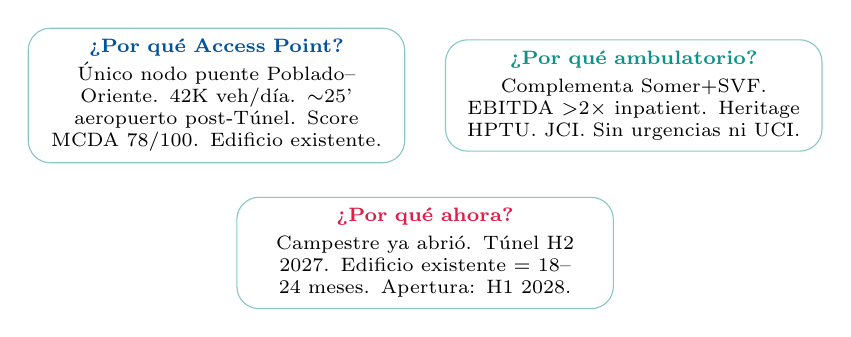
\begin{tikzpicture}[
  box/.style={draw=teal!50, fill=white, rounded corners=8pt,
              text width=4.5cm, minimum height=1.3cm, align=center,
              font=\scriptsize, inner sep=4pt},
]
\node[box] (why) at (0,0) {
  \textcolor{hptu}{\textbf{¿Por qué Access Point?}}\\[2pt]
  Único nodo puente Poblado--Oriente.
  42K veh/día. $\sim$25' aeropuerto post-Túnel.
  Score MCDA 78/100. Edificio existente.
};
\node[box] (what) at (5.3,0) {
  \textcolor{teal}{\textbf{¿Por qué ambulatorio?}}\\[2pt]
  Complementa Somer+SVF.
  EBITDA $>$2$\times$ inpatient.
  Heritage HPTU. JCI.
  Sin urgencias ni UCI.
};
\node[box] (when) at (2.65,-2.0) {
  \textcolor{rose}{\textbf{¿Por qué ahora?}}\\[2pt]
  Campestre ya abrió. Túnel H2 2027.
  Edificio existente = 18--24 meses.
  Apertura: H1 2028.
};
\end{tikzpicture}
\end{center}

\vspace{1pt}
\begin{exampleblock}{}
\centering
\highlight{Recomendación: sede ambulatoria HPTU en Access Point, Km 7 Vía Las Palmas}
\end{exampleblock}

\vspace{0pt}
{\tiny\textbf{¿Por qué no El Poblado?} Torre Oviedo, Rosario Tesoro, CEDIMED, BlueCare ya presentes. AP captura \highlight{ambos mercados}: Poblado + 298K Oriente.}
\end{frame}
}

% ---- LO QUE NO SABEMOS ----
{
\setbeamercolor{background canvas}{bg=amber!3}
\begin{frame}{Lo que NO sabemos (aún)}
\vspace{-2pt}
{\tiny
\begin{tabular}{@{}p{5.5cm}cp{5cm}@{}}
\toprule
\textbf{Pregunta abierta} & \textbf{Status} & \textbf{Próximo paso} \\
\midrule
\rowcolor{amber!8}
¿Acierto Inmobiliario quiere inquilino médico? & Pendiente & Reunión exploratoria --- abril 2026 \\
¿Edificio soporta MRI (15 ton) y quirófanos? & Pendiente & Inspección estructural \\
\rowcolor{amber!8}
¿SURA contrataría la sede ambulatoria? & Pendiente & Sondeo con dirección de red \\
¿Pacientes elegirían Km 7 sobre opciones locales? & Pendiente & Encuestas de intención \\
\rowcolor{amber!8}
¿Túnel 2da etapa llega en H2 2027? & Riesgo & Monitoreo trimestral ANI \\
¿Estratos Oriente son dato real o proxy? & Parcial & Solicitar datos a alcaldías \\
\bottomrule
\end{tabular}
}

\vspace{3pt}
\begin{exampleblock}{\small La recomendación se sostiene --- con condiciones}
\scriptsize
AP es la recomendación: \textbf{edificio existente} (18--24 meses) + \textbf{298K hab Oriente}. Condicionada a: (1) factibilidad estructural, (2) acuerdo con Acierto Inmobiliario, (3) pre-acuerdo aseguradora.
\end{exampleblock}

{\tiny\textcolor{amber!80!black}{\textbf{Transparencia:}} presentamos lo que sabemos y lo que no. Toda inversión tiene supuestos --- estos son los nuestros.}
\end{frame}
}

% ---- PRÓXIMOS PASOS ----
\begin{frame}{Próximos pasos}
\begin{center}
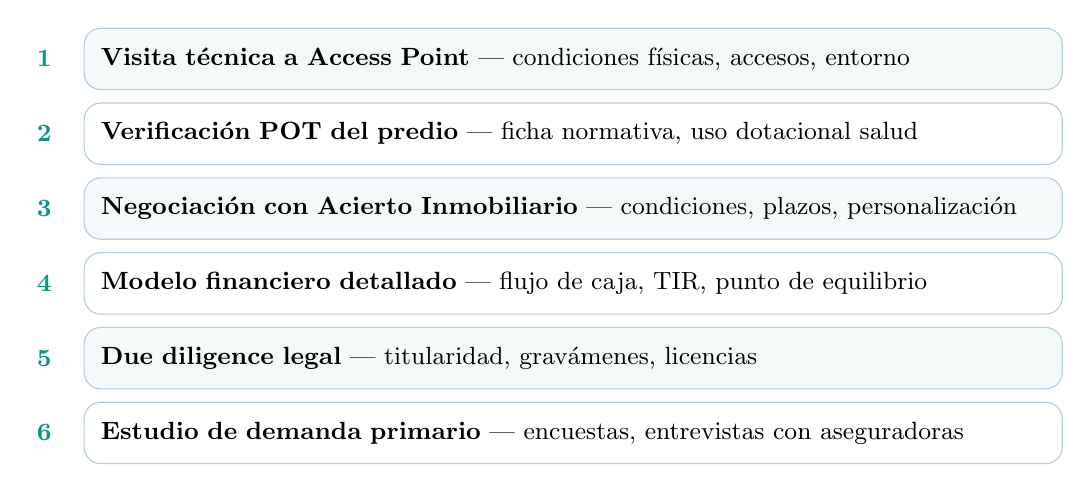
\begin{tikzpicture}[
  stepbox/.style={draw=hptu!30, fill=white, rounded corners=6pt,
              text width=12cm, minimum height=0.78cm, align=left,
              font=\small, inner sep=6pt},
  num/.style={font=\small\bfseries, teal, anchor=east},
]
\node[stepbox, fill=teal!5] (s1) at (0,0) {\textbf{Visita técnica a Access Point} --- condiciones físicas, accesos, entorno};
\node[num] at (-6.5,0) {1};
\node[stepbox] (s2) at (0,-0.95) {\textbf{Verificación POT del predio} --- ficha normativa, uso dotacional salud};
\node[num] at (-6.5,-0.95) {2};
\node[stepbox, fill=teal!5] (s3) at (0,-1.9) {\textbf{Negociación con Acierto Inmobiliario} --- condiciones, plazos, personalización};
\node[num] at (-6.5,-1.9) {3};
\node[stepbox] (s4) at (0,-2.85) {\textbf{Modelo financiero detallado} --- flujo de caja, TIR, punto de equilibrio};
\node[num] at (-6.5,-2.85) {4};
\node[stepbox, fill=teal!5] (s5) at (0,-3.8) {\textbf{Due diligence legal} --- titularidad, gravámenes, licencias};
\node[num] at (-6.5,-3.8) {5};
\node[stepbox] (s6) at (0,-4.75) {\textbf{Estudio de demanda primario} --- encuestas, entrevistas con aseguradoras};
\node[num] at (-6.5,-4.75) {6};
\end{tikzpicture}
\end{center}
\vspace{4pt}
{\footnotesize\textcolor{slate}{Pasos 1-3: abril 2026. Pasos 4-6: mayo-junio 2026. Decisión final: julio 2026.}}
\end{frame}

% ---- CIERRE ----
{
\setbeamercolor{background canvas}{bg=hptu}
\begin{frame}[plain]
\vfill
\begin{center}
{\Huge\bfseries\textcolor{white}{Plan de Expansión HPTU}}

\vspace{12pt}
{\Large\textcolor{white!85}{Sede Ambulatoria en Access Point}}

\vspace{20pt}
\begin{tikzpicture}
  \draw[white, line width=0.5pt] (0,0) -- (8,0);
\end{tikzpicture}

\vspace{14pt}
{\normalsize\textcolor{white!70}{MCDA 78/100 $\cdot$ 5 dimensiones $\cdot$ 3,000 simulaciones Monte Carlo}}

\vspace{6pt}
{\normalsize\textcolor{white!70}{CAPEX: COP \$67,000M $\cdot$ Revenue: \$51,000M $\cdot$ EBITDA: \$9,200M}}

\vspace{6pt}
{\normalsize\textcolor{white!70}{Payback: 6--8 años $\cdot$ Apertura: H1 2028}}

\vspace{6pt}
{\normalsize\textcolor{white!60}{Sin urgencias $\cdot$ Sin camas $\cdot$ Sin alta complejidad}}

\vspace{20pt}
{\small\textcolor{white!50}{Dashboard: hptu-localizacion.vercel.app}}

\vspace{14pt}
{\footnotesize\textcolor{white!40}{Abril 2026 $\cdot$ Presentación Completa}}
\end{center}
\begin{tikzpicture}[remember picture, overlay]
  \node[anchor=south] at ([yshift=14pt]current page.south) {
    
\includegraphics[height=1.2cm]{basica-white.png}
  };
\end{tikzpicture}
\vfill
\end{frame}
}

\end{document}
